% ######################################################################################################################
%         Placement-Factorization
% ######################################################################################################################

\chapter{Placement-Factorization}
\label{ch:Factorization}

\paperbox{
    This chapter is based on the peer-reviewed publication:
}{\paperpppp}{
    \textbf{Contributions:} Lucas Czech... Alexandros Stamatakis...
    \todo{}
}

% \todo{distance measures, nhd, simulations, mantel test}

% ######################################################################################################################
%         Background and Motivation
% ######################################################################################################################

\section{Background and Motivation}
\label{ch:Factorization:sec:Motivation}

Phylofactorization is a method to identify edges in a phylogenetic tree
that drive patterns in the composition of microbial communities \cite{Washburne2017a}.
An edge constitutes a separation or split of groups of taxa into the two subtrees induced by the edge.
In an evolutionary context, an edge denotes a difference in (putative) traits that may have arisen along the edge.
That is, an edge might describe characteristics and traits
that are only present in the set of taxa on one side of the edge, but not in the set on the other side.
The goal of Phylofactorization is to identify edges that are related to differences in per-sample meta-data features.
% That is, it finds groups of taxa for which a change in abundances is reflected in changes in environmental variables.
To this end, it aggregates and contrasts the abundances in the subtrees (groups of taxa) induced by an edge,
and evaluates how changes in environmental variables across samples are reflected in abundance changes.

The original method \cite{Washburne2017a} uses a tree inferred from the OTUs that are present in the set of samples,
% and represents each sample by its OTU abundances at the tips of the tree.
% Each edge splits the tree, and thus induces clades that correspond to sets of OTUs,
% which are called \emph{binned phylogenetic units} (BPUs) in this context.
and iteratively identifies edges that split the tree into nested subtrees
which exhibit the largest predictable differences between the taxa in these subtrees.
Each such edge can be interpreted as a \emph{phylogenetic factor} (or short, \emph{phylofactor}) for splitting the tree:
Once an edge has been selected in one iteration, its induced subtrees are then considered separately in subsequent iterations.
The resulting factors are hence independent of each other, which ensures orthogonality of the factors.
In other words, each factor describes a different dimension in which samples differ. %, analogous to Edge PCA.
Furthermore, by iteratively considering subtrees of decreasing size, nested factors can be found,
which correspond to relationships within a subtree that only affect the taxa in the subtree itself.
The algorithm stops after a predefined number of iterations/factors, %(that is, until a certain number of edges have been found),
or until a stopping criterion is met.

In a typical use case, each environmental sample is represented by its OTU abundances at the tips of the tree,
that is, by counts of how often each OTU is present in the sample; 
see \secref{ch:Foundations:sec:SequenceAnalysis:sub:OTUs} for details on OTUs of metagenomic samples.
Given a per-sample meta-data feature such as the pH-value,
Phylofactorization can then be employed to find edges where a change of the pH-value between samples
predicts a change in OTU abundances in the two subtrees induced by the edge.
For example, an increasing ph-value might indicate
a relative increase in the OTU abundances in one subtree compared to another subtree.
The resulting factorization can serve as a dimensionality-reduction mechanism, as an ordination and visualization tool,
and as an inferential tool that can identify edges corresponding to changes in functional ecological traits \cite{Washburne2017a}.
We later showcase some of these applications in \secref{ch:Factorization:sec:Evaluation}.

% ######################################################################################################################
%         Methods and Implementation
% ######################################################################################################################

\section{Methods and Implementation}
\label{ch:Factorization:sec:Methods}

We here present an adaptation of Phylofactorization to phylogenetic placements, which we call \emph{Placement-Factorization}.
We explain our adaptation following the description of the Generalized Phylogenetic Factorization (GPF) \cite{Washburne2018,Washburne2019}.
The GPF is a recent generalization of Phylofactorization
that also allows for types of input data other than relative OTU abundances, for example, presence/absence data.
It is hence suited for a wider range of community ecological data \cite{Washburne2019}.
Conceptually and algorithmically, Phylofactorization, GPF, and our Placement-Factorization, work the same;
we here use the mathematical notation of GPF as a scaffold to explain our adaptation.
In the following, we briefly introduce the original method, outline the necessary adaptations,
and explain how to use the balances obtained from (our adaptation of)
the PhILR transform (as explained in \chpref{ch:Balances}) in the context of Placement-Factorization.

% ======================================================================================================================
%     Placement Factorization
% ======================================================================================================================

\subsection{Placement-Factorization}
\label{sec:Factorization:sub:Methods:sub:Phylofactor}

Phylofactorization can be understood as an iterative greedy graph-partitioning algorithm for a tree $T$ \cite{Washburne2018}.
In each iteration, a \emph{winning edge} $e^*$ is identified
that splits edges of the tree into two disjoint groups $R$ and $S$.
To determine the winning edge, an \emph{objective function} is maximized
that expresses the intensity of the relationship between abundances and meta-data variables.
We later discuss this objective function in more detail in \secref{sec:Factorization:sub:Methods:sub:ObjectiveFunction}.

% ------------------------------------------------
%     Input
% ------------------------------------------------

\paragraph{Input}
\label{sec:Factorization:sub:Methods:sub:Phylofactor:par:Input}

The input to the original Phylofactorization is an $n \times m$ data matrix $X$,
containing $j = 1, \ldots, n$ samples, and $i = 1, \ldots, m$ species (corresponding to the OTUs at the tips of the tree).
The values of the matrix can represent abundances, presence/absence data, 
or other data related to the species in the tree \cite{Washburne2019}.

In our adaptation, we use the per-edge masses from the phylogenetic placement of the samples.
% (disregarding that the matrix is transposed here compared to the notation used there).
That is, instead of $m$ species representing the tips of the tree,
we use an $n \times m$ data matrix $X$ where the $m$ columns correspond to the edges of our reference tree
(for consistency of notation, we re-use and re-purpose the index $m$ here,
and transpose $X$ compared to the original notation).
This is again the mass matrix that we used in the previous methods (\chpref{ch:Visualization} and \chpref{ch:Clustering}),
and which we showed before in \figref{fig:masses_imbalances:sub:Matrices} and \figref{fig:balances:sub:masses}.

Lastly, Phylofactorization uses an $n \times p$ meta-data matrix $Z$ for the $n$ samples
and $p$ per-sample meta-data variables.
This is the same meta-data matrix that we used for example in Edge Correlation
(\secref{ch:Visualization:sec:Methods:sub:EdgeCorrelation}) and showed in \figref{fig:masses_imbalances:sub:Matrices}.

% ------------------------------------------------
%     Algorithm
% ------------------------------------------------

\paragraph{Algorithm}
\label{sec:Factorization:sub:Methods:sub:Phylofactor:par:Algorithm}

In analogy to the Generalized Phylofactorization \cite{Washburne2018,Washburne2019},
our adapted algorithm requires three functions:

\begin{enumerate}
    \item An \emph{aggregation function} $A_R = A( X_{j,R}, ~T )$,
          which aggregates (summarizes) a subset $R$ of edges for a sample $j$.
    \item A \emph{contrast function} $C_{R,S} = C( A_R, ~A_S, ~T, ~e )$, which contrasts (compares)
          the aggregates of two disjoint subsets $R$ and $S$ of edges on the two sides induced by an edge $e$.
          % C( A( X_{j,R}, T ), A( x_{j,S}, T ), T, e )
    \item An \emph{objective function} $\omega(C, ~Z)$ that evaluates a contrast for all samples
%          (for example, the contrast between groups $R$ and $S$ induced by a given edge)
          in the context of the per-sample meta-data, in order to determine the winning edge.
\end{enumerate}

We later discuss appropriate choices for these functions.
For now, we assume that we are given functions that allow identifying edges
whose induced subtrees exhibit predictable differences in the edge masses $X$
driven by changes in the meta-data $Z$ of different samples.
The algorithm starts by considering the entire tree $T$ as one large ``subtree''.
Then, in each iteration, Phylofactorization and Placement-Factorization work as follows:

\begin{enumerate}
    \item For each edge $e$ that separates disjoint groups $R_e$ and $S_e$ of edges within the subtree that contains $e$:
          \begin{enumerate}
              \item Compute the aggregates $A_{R_e} = A( X_{j,R_e}, ~T )$ and $A_{S_e} = A( X_{j,S_e}, ~T )$.
              \item Compute their contrast $C_e = C( A_{R_e}, ~A_{S_e}, ~T, ~e )$. %$C_{R_e, S_e}$.
              \item Compute the objective value $\omega_e = \omega(C_e, ~Z)$.
          \end{enumerate}
          The aggregates $A_{R_e}$ and $A_{S_e}$, as well as the contrast $C_e$ are computed separately for every sample.
          The value $\omega_e$ of the objective function then expresses the relationship of the contrasts of all samples
          with their respective meta-data values in $Z$.
    \item Select the winning edge $e^* = \argmax_e ( \omega_e )$ that maximizes the value of the objective function.
    \item Partition the subtree that contains the winning edge $e^*$ into two disjoint subtrees, separated by $e^*$.
    \item Repeat until a stopping criterion is met.
\end{enumerate}

This closely follows the description of the algorithm in \cite{Washburne2018,Washburne2019}, see there for details.
The difference between the algorithms is that the groups $R$ and $S$ in our case consist of reference tree edges,
instead of species at the tips of the OTU tree.
Because of this, the aggregates of edges that lead to tip nodes are empty,
meaning that we do not consider those edges as candidates in the algorithm.
This is analogous to ``tip edges'' not having a meaningful edge imbalance, 
as described in \secref{ch:Foundations:sec:PhylogeneticPlacement:sub:PlacementProcessing:par:EdgeImbalances}.
An example of the first two iterations of the algorithm is shown in \figref{fig:phylofactor}.

\begin{figure}[!htbp]
    \centering
    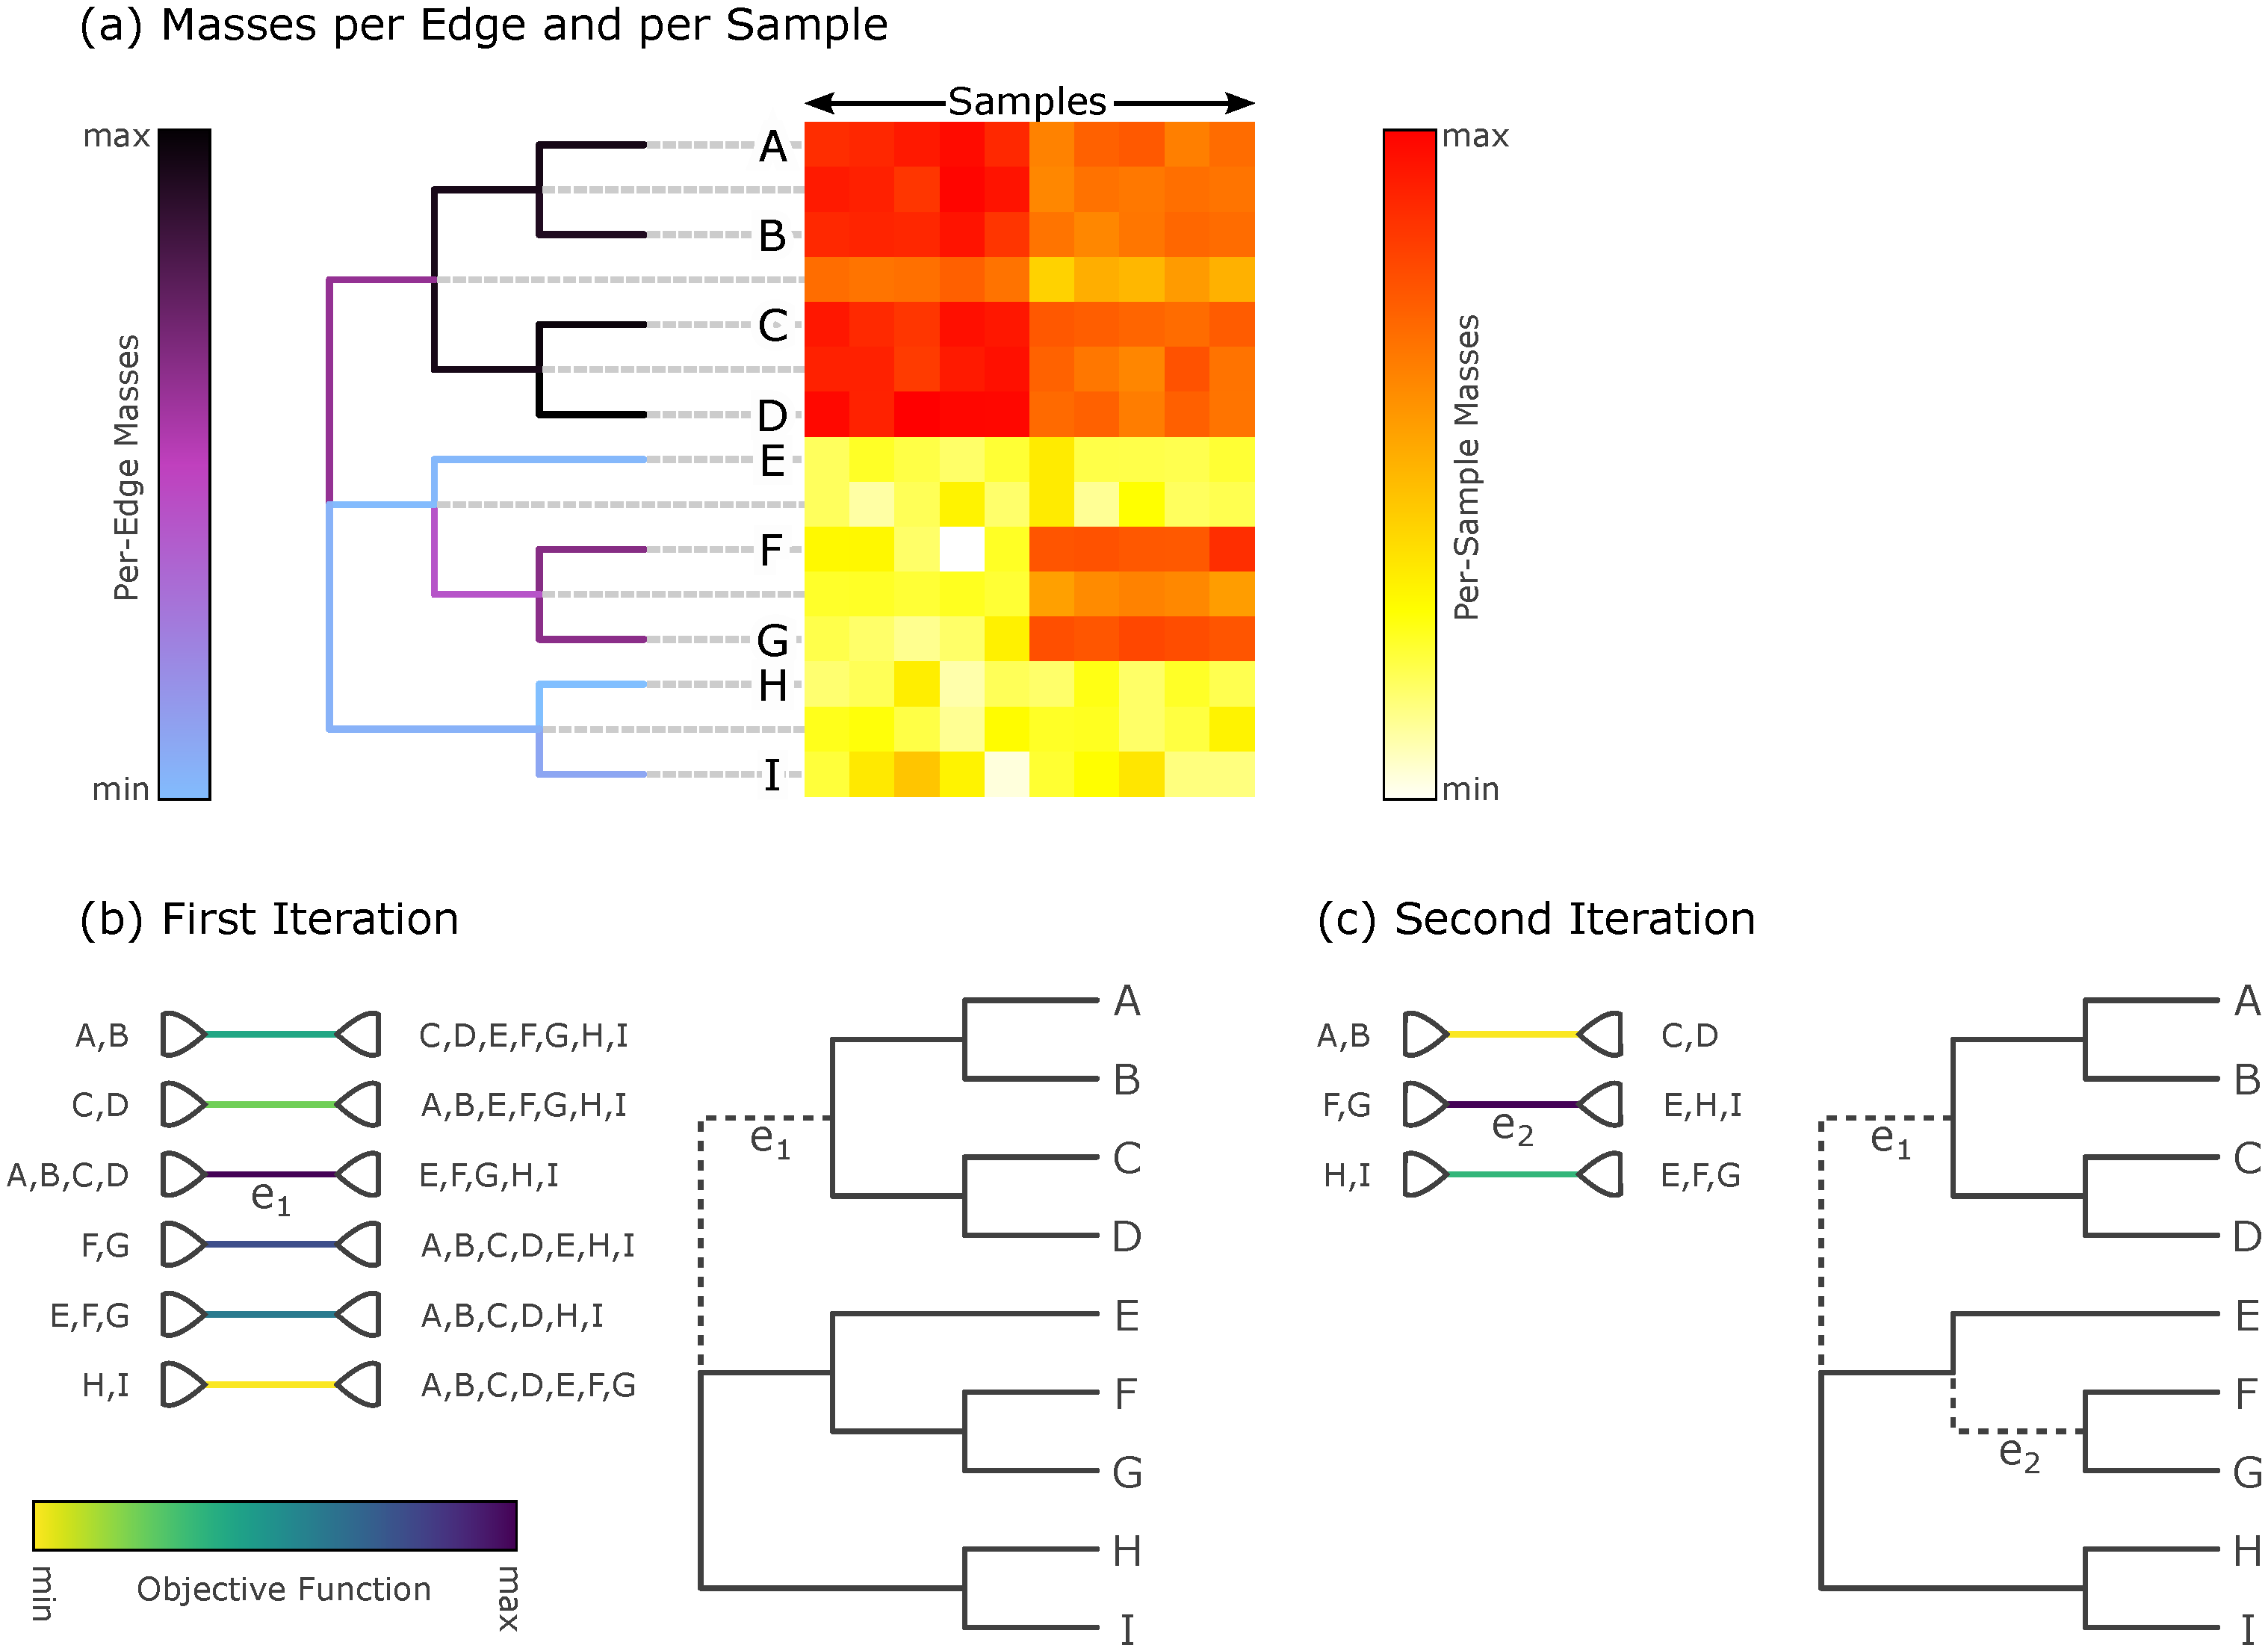
\includegraphics[width=\linewidth]{pdf/phylofactor.pdf}
    \begin{subfigure}{0pt}
        \phantomcaption
        \label{fig:phylofactor:sub:heat_tree}
    \end{subfigure}
    \begin{subfigure}{0pt}
        \phantomcaption
        \label{fig:phylofactor:sub:first}
    \end{subfigure}
    \begin{subfigure}{0pt}
        \phantomcaption
        \label{fig:phylofactor:sub:second}
    \end{subfigure}
    \caption[Input data and first two iterations of Placement-Factorization]{
        \textbf{Input data and first two iterations of Placement-Factorization.}
        The figure resembles Figure~2 of \citeay{Washburne2017a}.
        It shows the adaptation of concepts from Phylofactorization to phylogenetic placement data.
        \\
        \subref{fig:phylofactor:sub:heat_tree}
        The input data is a set of samples with placement masses on each edge of the tree.
        The tree is colorized by the total mass across all samples, that is, by the row sums of the heat map.
        The heat map then shows the detailed mass per edge (rows) and per sample (columns),
        and hence is an example of the mass matrix of \figref{fig:masses_imbalances:sub:Matrices}.
        Note that the heat map also contains rows for each inner edge of the tree,
        as phylogenetic placement also considers these edges.
        This is different from OTU abundance heat maps that only have entries for the tips of the tree.
        We show a further example of this visualization for empirical data in \figref{fig:heat_tree}.
        \\
        \subref{fig:phylofactor:sub:first} In the first iteration,
        the objective function for all inner edges is evaluated.
        Here, edge $e_1$ is the winning edge that maximizes the objective function,
        which separates the clade ({\sffamily A}, {\sffamily B}, {\sffamily C}, {\sffamily D}) from the rest of the tree.
        \\
        \subref{fig:phylofactor:sub:second} In the second iteration,
        only the contrasts within the two subtrees %(orange and black)
        are calculated,
        but not across the winning edges of previous iterations (here, $e_1$).
        That is, the winning edge $e_2$ maximizes the objective function that contrasts clade ({\sffamily F}, {\sffamily G})
        with clade ({\sffamily E}, {\sffamily H}, {\sffamily I}),
        but does not consider the edges in the subtree ({\sffamily A}, {\sffamily B}, {\sffamily C}, {\sffamily D}).
        Note that in our adaption, edges that lead to a tree tip are not considered as potential factors.
    }
    \label{fig:phylofactor}
\end{figure}

Each iteration further splits a subtree at the respective winning edge,
so that after $i$ iterations, $i+1$ subtrees are produced.
It is important to note that the winning edges of previous iterations split the tree into \emph{disjoint} subtrees,
and that in later iterations,
the aggregates and contrasts induced by an edge are only computed \emph{within} their respective subtrees.
This ensures the previously mentioned orthogonality of the phylogenetic factors (winning edges),
meaning that systematic dependencies between the contrasts of any two factors are eliminated,
and that instead, nested relationships can be identified.

The original publication proposes a stopping criterion using a Kolmogorov-Smirnov (KS) test \cite{Massey1951}
based on % (significance levels of)
test statistics of the identified phylofactors \cite{Washburne2017a,Washburne2019}.
Although these could be implemented for Placement-Factorization, we leave this as future work;
our implementation currently runs for a given number $i$ of iterations, and hence computes $i$ phylofactors.
% We leave elaborate stopping criteria as future work.
% based on a Kolmogorov-Smirnov (KS) test of the distribution of P-values from analyses of variance of the regressions on candidate ILR coordinates.

So far, we have assumed to be given the three functions required for Phylofactorization.
The choice of these functions depends on the data $X$, the data $Z$, and the research question at hand.
In order to be consistent and comparable with the original implementation \cite{Washburne2017a},
in our evaluation we used the same set of functions,
namely the balances of the ILR transformation as explained in \chpref{ch:Balances} for aggregating and contrasting subtrees,
and an objective function based on \acfp{GLM}, 
which we explain in the following, 
see \secref{sec:Factorization:sub:Methods:sub:ObjectiveFunction} and \secref{sec:Factorization:sub:Methods:sub:GLMs}.

% ------------------------------------------------
%     Output
% ------------------------------------------------

\paragraph{Output}
\label{sec:Factorization:sub:Methods:sub:Phylofactor:par:Output}

The main output of the algorithm is the list of winning edges, that is, 
of the phylogenetic factors that have been identified.
% These can for example be visualized directly as coloured clades on the tree.
Furthermore, one can store detailled tables with the balances per sample for all factors,
the values of the objective function at each edge for all factors,
as well as much more intermediary data of the algorithm.
We later show examples of how these outputs can be used for analysis and visualization purposes
in \secref{ch:Factorization:sec:Evaluation}.

% Not relevant any more:
% For our adaptation, %of Phylofactorization to phylogenetic placement data,
% a straight-forward choice could for instance be the following:
% To aggregate a group of edges, their per-edge placement mass is summed up;
% to contrast two aggregates, their difference is taken;
% to evaluate a contrast (objective function), the correlation with per-sample meta-data is calculated.
% This choice of functions would basically be identical to using \nameref{sec:Introduction:sub:Imbalances}
% and \nameref{sec:MaterialsMethods:sub:Visualization:sub:Correlation} constrained to the subtrees of the factors,
% and would yield phylofactors that are consistent with these approaches.
% % \todo{should we also eval this? probably yes... will see if there is time.}
% % \todo{this might have downsides that should be explored fist, and we should test it, etc...
% % but at least mention that this is not the best choice, and why GLMs are better}
% However, in order to be consistent and comparable with the original implementation \cite{Washburne2017a},
% in our evaluation we used the same set of functions,
% namely the balances of the ILR transformation as explained above for aggregating and contrasting subtrees,
% and an objective function based on \acfp{GLM}, which we explain in the following.
% % In the following,

% Back from when the order of sections was different:
% In the following sections, we describe alternative choices for these functions,
% based on the suggestions of \cite{Silverman2017} and \cite{Washburne2017a}:
% First, we introduce the ILR Transform and balances, which can be used for aggregation and contrasting.
% We further consider a weighting scheme for taxa/edges with low abundance/mass.
% We then discuss the choice of the objective function in more detail,
% and explain how Generalized Linear Models can be employed to this end.
% In each section, we also explain the changes that are necessary
% in order to adapt these approaches to phylogenetic placements.
% Finally, we bring these concepts together by explaining how to use them
% for Phylofactorization in the context of phylogenetic placement.
% and elaborate on their advantages compared to other choices of functions.

% ======================================================================================================================
%     Objective Function
% ======================================================================================================================

\subsection{Objective Function}
\label{sec:Factorization:sub:Methods:sub:ObjectiveFunction}

% Phylofactorization requires an objective function $\omega(C, ~Z)$ that selects the winning edge $e^*$ of each iteration
% based on (i) the contrasts $C$ between the two subtrees induced by all edges, and (b) the meta-data variables in $Z$.
% The choice of objective function depends on the research question at hand;
% see \cite{Washburne2017a} and \cite{Washburne2018} for a thorough discussion.
% Typically, an appropriate objective function quantifies some form of relationship between $C$ and $Z$,
% for example, the variation in $C$ explained by regression on $Z$, or some other measure of correlation between the two.

Phylofactorization requires an objective function $\omega(C_e, ~Z)$
that quantifies the relationship between $C_e$ and $Z$ for a given edge $e$,
where $C_e$ are the contrasts between the two subtrees induced by $e$ for all samples (for example, the balances),
and $Z$ are the per-sample meta-data variables.
That is, both $C_e$ and $Z$ have size $n$, the number of samples,
with $Z$ potentially containing multiple columns (one for each meta-data feature).
In order to identify the winning edge $e^*$ of an iteration (the \emph{phylofactor}),
the function is evaluated for all edges, and the edge maximizing $\omega$ is selected.
The choice of the objective function depends on the research question at hand;
see \citeay{Washburne2017a} and \citeay{Washburne2018} for a thorough discussion.

Our implementation is as general as the original Phylofactorization \cite{Washburne2017a},
in that it allows for an arbitrary objective function.
For simplicity, and in line with the original publication,
we here focus on functions that treat the meta-data variables $Z$ as independent variables
and the contrasts $C_e$ as dependent variables whose relationship with $Z$ is assessed, for instance, via a predictive model.
Then, the selected phylogenetic factors correspond to edges
where a change in $Z$ most strongly predicts a change in $C_e$ across the samples,
that is, where the effect of the (independent) meta-data variables
on the (dependent) underlying data (e.g., per-clade abundances) is most pronounced.

% A simple starting point is to use the magnitude of correlation between $C_e$ and $Z$ as objective function.
% This is easy to compute and yields phylofactors that are consistent with our previously described in
% \nameref{sec:MaterialsMethods:sub:Visualization:sub:Correlation},
% and can reveal correlations at deeper, nested levels of the underlying tree.
% \todo{maybe refer to results/supplement for this, if we make any of this.}
% This however only allows for a single column (one meta-data feature) in $Z$,
% and does not work well with balances, as we show in our evaluation
% \todo{rephrase: and entails certain issues}
% \todo{maybe remove this part}.
% Furthermore, because the magnitude of the correlation has to be used
% in order for the maximization of the objective function to work,
% the direction of the correlation is lost.

% ------------------------------------------------
%     Generalized Linear Models
% ------------------------------------------------

\paragraph{Generalized Linear Models}
\label{sec:Factorization:sub:Methods:sub:ObjectiveFunction:par:GLMs}

A powerful approach is to model the relationship between $C_e$ and $Z$ via linear regression,
that is, we assess how well $Z$ can predict $C_e$.
In the simple one-dimensional case, this can be thought of as fitting a line through a scatter plot
of the meta-data feature on the $x$-axis and the contrasts on the $y$-axis, where each point represents one sample.
This concept is generalized via \acfp{GLM} \cite{Nelder1972,McCullagh1989,Agresti2018}.
% We here provide a brief intuition about \acp{GLM}; for details see \cite{McCullagh1989} and \cite{Agresti2018}.
% We provide a brief introduction to \acp{GLM} in S3~Text; for details see \cite{McCullagh1989} and \cite{Agresti2018}.
% \todo{Will have to see whether I can finish this in time. If not, remove the above. The explanation here should be enough for now.}

We introduce \acp{GLM} in more detail in \secref{sec:Factorization:sub:Methods:sub:GLMs}.
In short, \acp{GLM} allow to predict a single (response) variable using multiple input (explanatory) variables.
Typically, the response variable is assumed to follow any distribution from the exponential family
(normal, exponential, Poisson, Binomial, etc.), which is given for balances as used here.
In contrast to this, the explanatory variables (the meta-data features)
are assumed to have a linear relationship with the response.
%, while the explanatory variables are assumed to be linear --> but transformation allows to use any input really.
Note that this mathematical restriction of the model does not mean
that only meta-data features can be used that behave linearly;
transformations and interactions of the features basically allow for arbitrary types of data.
For example, categorical variables such as the body site where a sample was taken from can be transformed
into so-called dummy variables that fulfill the requirements.
% We later use this for the \ac{HMP} dataset, see \secref{sec:Results:sub:Phylofactor:sub:HMPDataset}.

Once the model parameters of the \ac{GLM} have been estimated,
that is, once it has been fit to the data via some optimization algorithm,
% The most commonly used is the iteratively reweighted least squares (IRLS) method \cite{Burrus2012},
% which yields a maximum likelihood estimation of the model parameters, and which is what we use in our implementation.
we need to evaluate the \ac{GLM} for the purposes of Phylofactorization.
We are interested in a value for $\omega$ that expresses how well the meta-data variables explain the balances.
To this end, Phylofactorization and our adaptation thereof use the difference between the null deviance of the balances
and the deviance obtained from the \ac{GLM}.
% The null deviance can be understood as the deviation from the mean value of the balances.
This difference %between null deviance and deviance of the model
expresses how much better the model explains the balances than just predicting them from their mean.
For details on the usage of \acp{GLM} for Phylofactorization, see \cite{Washburne2017a}.

% In S3~Text, we also describe %how to assess how well a \ac{GLM} fits/predicts the data,
% how to evaluate a \ac{GLM} for our purposes here, that is, how to use it to obtain a value for $\omega$.

% ------------------------------------------------
%     Usage in Phylofactorization
% ------------------------------------------------

\paragraph{Usage in Phylofactorization}
\label{sec:Factorization:sub:Methods:sub:ObjectiveFunction:par:Usage}

Predictive models such as \acp{GLM} expect the response variable (that is, the predicted values; here, the contrasts)
to have certain statistical properties.
In particular, linear models assume the deviation of response from the predicted value to be normally distributed.
The ILR transform for compositional data has been proven to behave asymptotically normal \cite{Egozcue2003,Pawlowsky-Glahn2011a},
which allows their application within standard multivariate methods,
and within \acp{GLM} as presented here.
% and to Phylofactorization and Placement-Factorization as presented here.

Lastly, we note that depending on the research question, other objective functions can be used,
see \cite{Washburne2017a,Washburne2018} for some examples.
For instance, simple test statistics such as the variation in $C_e$ explained by regression on $Z$ can be used.
Furthermore, instead of predicting contrasts from meta-data, one could be interested in the opposite,
that is, predicting a meta-data variable given the per-sample contrasts.
In this case, the maximization of the objective function yields edges that best predict a certain feature of the data;
this is suitable for identifying clades that can serve as a bio-indicator.
Using \acp{GLM} for this allows to model any type of meta-data variable;
for example, the binary information encoded in presence/absence data can be predicted using logistic regression.
While our implementation supports all those use cases,
they have been explored and discussed before \cite{Washburne2017a,Washburne2019}.
For the sake of simplicity, we focus on linear (gaussian) modeling of $C_e \sim Z$,
that is, predicting balances from meta-data.

% ======================================================================================================================
%     Generalized Linear Models
% ======================================================================================================================

\subsection{Generalized Linear Models}
\label{sec:Factorization:sub:Methods:sub:GLMs}

We here take a short digression to introduce \acfp{GLM}


This concept is generalized even further by a \acf{GLM} \cite{Nelder1972,McCullagh1989}.
We here provide a brief intuition about \acp{GLM}; for details see \cite{McCullagh1989} and \cite{Agresti2018}.


% Sources:
% https://en.wikipedia.org/wiki/Generalized_linear_model
% https://newonlinecourses.science.psu.edu/stat504/node/216/
% http://www.stat.cmu.edu/~ryantibs/advmethods/notes/glm.pdf

In the context of \acp{GLM},
the independent variables (e.\,g., $Z$) are called the \emph{predictor variables} or \emph{explanatory variables},
while the dependent variable (e.\,g., $C_e$) is called the \emph{response variable}.
\acp{GLM} generalize from linear regression by allowing
(a) for the response variable to have an arbitrary distribution
(instead of a normal distribution, which is implicitly assumed in linear regression),
and (b) for an arbitrary function of the response variable (called the \emph{link function})
to vary linearly with the predicted values (instead of the response variable itself varying linearly).
%  by allowing the magnitude of the variance of each measurement to be a function of its predicted value
% we here briefly describe the gaussian 1d case in order to provide some intuition about linear models
% here, we describe the simple linear case of using metadata to predict contrasts (which can for example be balances, as described above)

% ------------------------------------------------
%     Overview
% ------------------------------------------------

\paragraph{Overview}
\label{sec:Factorization:sub:Methods:sub:GLMs:par:Overview}

We here use the standard notation of $X$ being the predictor of size $n \times p$ and $Y$ being the response of size $n$,
with $n$ the number of data points (samples) and $p$ the number of predictor variables.
Then, a \ac{GLM} is described by three components \cite{McCullagh1989}:
a \emph{random component}, a \emph{systematic component}, and \emph{link component}.

The \emph{random component} specifies the probability distribution of $Y$ (conditioned on $X$);
also called the \emph{error} or \emph{noise model}.
For example, in linear regression, we assume $Y$ to deviate from the prediction by a normally distributed error,
while in logistic regression, the deviation is assumed to be binomially distributed.

The \emph{systematic component} specifies the linear combination $\eta$ of the predictors $X$
using the (unknown) parameters $\beta$:
\begin{equation}
% \label{ch:MaterialsMethods:sec:BalancesPhyloFactors:eq:eta}
\label{supp:sec:GLM:eq:eta}
    \eta ~:=~ \beta_0 + \beta_1 X_1 + \dots + \beta_p X_p
\end{equation}
This is the ``linear'' part of the model.

The \emph{link component} connects the random and systematic components via an invertible link function $g$.
In particular, the link function provides a connection between the expected value $\mathbb{E}$ of $Y$ and $\eta$:
\begin{equation}
% \label{ch:MaterialsMethods:sec:BalancesPhyloFactors:eq:link}
\label{supp:sec:GLM:eq:link}
    % g(\mu) ~=~ \eta
    g(\mathbb{E}(Y)) ~=~ \eta
\end{equation}
If the distribution of $Y$ (the random component) is assumed to be a member of the exponential family of distributions,
there is a \emph{canonical} link function for each member of the family.
For example, for the normal distribution, $g$ is the identity function,
while for a binomial distribution, $g$ is often the logit (log-odds) function.

The expected value is usually estimated as the mean of $Y$, meaning that $\mathbb{E}(Y) = \mu$.
\todo{is that the correct wording?}
The full model is then given by:

\begin{equation}
%     \label{ch:MaterialsMethods:sec:BalancesPhyloFactors:eq:GLM}
    \label{supp:sec:GLM:eq:GLM}
    \mathbb{E}(Y) ~=~ \mu ~=~ g^{-1}(\eta) ~=~ g^{-1}( \beta_0 + \beta_1 X_1 + \dots + \beta_k X_p )
\end{equation}
% \begin{align}
%     \label{ch:MaterialsMethods:sec:BalancesPhyloFactors:eq:GLM-exp}
%     \mathbb{E}(Y) ~&=~ \mu \\
%     \label{ch:MaterialsMethods:sec:BalancesPhyloFactors:eq:GLM-link}
%     g(\mu) ~&=~ \beta_0 + \beta_1 X_1 + \dots + \beta_p X_p
% \end{align}

\todo{maybe use matrix notation here to state that this is done per sample?!}

The choice of distribution and link is typically informed by the type of data $Y$ that they are used for:
For example, if $Y$ is assumed to respond linearly, the normal distribution and the identity link are well suited;
if $Y$ are categorical data or counts (``yes''/``no'' choices), a binomial distribution and a logit link can be used;
and if $Y$ are counts of occurrences in a fixed amount of time, the Poisson distribution and a log link are typical.

\todo{add graphs with examples, such as logit and poisson, see } \verb|21121_Chapter_15.pdf|

can use many x of type binary or linear or transformation or factors

predict a single variable from multiple


how to fit? ML estimator for beta
typically, using the Iterative Reweighted Least Squares (IRLS) method \cite{Burrus2012}


connect


\begin{figure}[!htb]
    \centering
    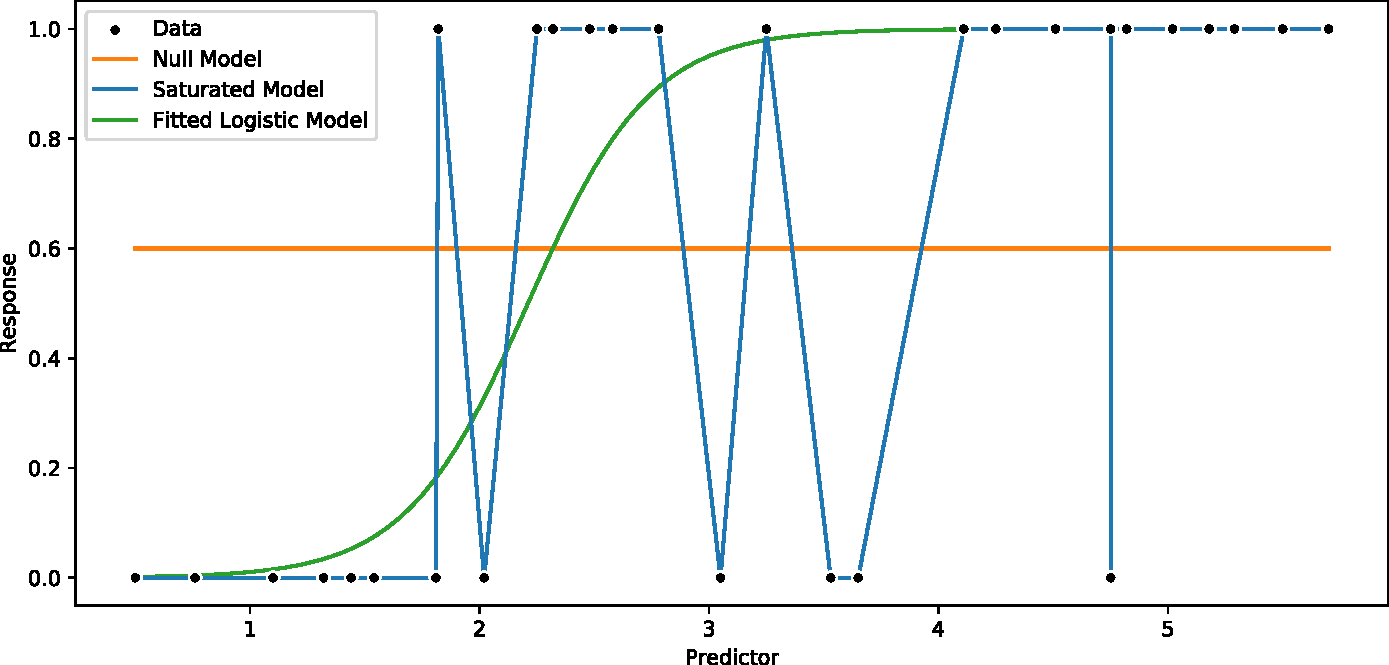
\includegraphics[width=\linewidth]{pdf/logistic_regression.pdf}
    \caption[Example of logistic regression]{
        \textbf{Example of logistic regression.}
        The data represents a continous predictor (explanatory) variable and a binary response variable;
        for example, the hours a student spent learning for an exam and whether the student passed (1) or failed (0) the exam.
        The null model only has a single parameter $\beta_0$ to predict the outcome;
        the optimum is hence to always predict the mean of the data.
        The saturated model on the other hand is able to predict each datum correctly,
        at the expense of model simplicity.
        Because of the binary response variable, a binomial logistic regression is a good model for the data:
        it attempts to fit the data using two parameters $\beta_0$ and $\beta_1$.
    }
    \label{fig:logistic_regression}
\end{figure}

% ------------------------------------------------
%     Different Types of Data
% ------------------------------------------------

\paragraph{Different Types of Data}
\label{sec:Factorization:sub:Methods:sub:GLMs:par:Data}

Depending on the assumption of the

\todo{figure: logistic regression, see } \verb|https://www.sagepub.com/sites/default/files/upm-binaries/21121_Chapter_15.pdf|
and \verb|https://bookdown.org/egarpor/SSS2-UC3M/logreg-deviance.html|
or \verb|https://www.stat.berkeley.edu/~blfang/STAT151A/STAT151A_lab11.html|


transformation of the input vars allows to use any input.

presence absence and categorical data can be encoded with dummy variables, that is as cols of 0 1

note that this does not mean that the relationship between the predictor variables (meta-data) and response variable (contrasts) has to be linear:
the predictor variables can be arbitrarily transformed, and
wiki:
and in fact multiple copies of the same underlying predictor variable can be added, each one transformed differently.
in order to model other types of relationships.
this is however out of scope.

so, both predictor vars and response var can be non linear, in a sense...
ion between glm and pearson

% ------------------------------------------------
%     Assessing the Fit of the Model
% ------------------------------------------------

\paragraph{Assessing the Fit of the Model}
\label{sec:Factorization:sub:Methods:sub:GLMs:par:Fitness}

introduce terminology: residuals

Model fit: R 2, residual analysis, F-statistic

the objective function for finding phylo factors:
we use the same as the paper, that is, null deviance minus residual deviance.
for glm, this is the difference in log likelihoods between the models.
in the case of a simple linear regression, which assumes normally distributed errors with constant variance,
the null deviance is the mean of squares from mean,
and the res dev is the mean of squares from the regression line.
we are hence using a simple linear regression of the meta-data feature on the balances.

intuitively, this measures how much better a linear function of the meta-data $Z$ is
for predicting the contrasts $C$ instead of just ``predicting'' the mean value.

this can be thought of as fitting a line through a plot of the the meta-data feature on the x-axis and the balance on the y-axis,
where each point represents one sample.
this is done for every edge of the tree
the objective is then to find the edge where the model (a simple linear model in our case) best explains the data,
that is, where the balances can be best predicted from the meta-data.
in the original publication [cite], they use GLMs and hence optimize an objective function that maximizes
the difference between null deviance and model deviance.

null deviance: LL of sat minus LL of null model. which in case of a linear regression model is the variance $\sigma^2$

\todo{go on about what that is, and how gaussian residuals with fixed variance are assumed, and density function, etc...}
in our simple linear regression, this simplifies to the difference between the variance of the balances
and the mean squared error obtain from the linear model:


%     \sigma^2

where $\bm{\hat{y}}$ are the estimates

\begin{align*}
%     \label{sec:MaterialsMethods:sub:BalancesPhyloFactors:eq:ObjectiveFunction}
    \label{supp:sec:GLM:eq:ObjectiveFunction}
%     \operatorname{VAR}(y) &= \frac{1}{n} \sum_{i=1}^{n} \left( y_i - \bar{y}_i \right)^2 \\
%     \operatorname{MSE}(y) &= \frac{1}{n} \sum_{i=1}^{n} \left( y_i - \hat{y}_i \right)^2
    O(\bm{y}) ~=~ \sigma^2(y) - \delta^2(y)
    ~=~ \frac{1}{n} \sum_{i=1}^{n} \left( y_i - \bar{y} \right)^2
    ~-~ \frac{1}{n} \sum_{i=1}^{n} \left( y_i - \hat{y}_i \right)^2
%     O &= \operatorname{VAR}(y) - \operatorname{MSE}(y) \\ \\
%       &= \frac{1}{n} \sum_{i=1}^{n} \left( y_i - \bar{y} \right)^2
%        - \frac{1}{n} \sum_{i=1}^{n} \left( y_i - \hat{y}_i \right)^2
\end{align*}

with $\bar{y}$ being the mean, and $\hat{y}_i$ being the residuals of the prediction,
that is, the deviations of each point from the regression line.

from \url{http://www.imm.dtu.dk/~hmad/GLM/slides/lect06.df}
For the normal distribution with $\Sigma = I$, the deviance is just the residual sum of squares (RSS).

this can be interpreted as follows: the null model is given by the variance of the balances around their mean,
which simply fits the intercept (mean) to the values, and can hence be seen as ``the data has that much dispersion''.
the mean squared error of the fitted linear model on the other hand tries to better explain the balances,
and is always less or equal to the variance, as the null model is a linear model with slope $0$.
this also means that these models are nested, and their (log) likelihoods can thus be compared,
which is what the difference between them expresses: high variance but low mse means: the data is not well explained
by its mean, but by the linear model. hence, maximizing this quantity in order to find the next phylo factor means:
we are looking for an edge that is best explained by a (linear) function of the meta-data.


% ------------------------------------------------
%     Usage of Balances in GLMs
% ------------------------------------------------

\paragraph{Usage of Balances in GLMs}
\label{sec:Factorization:sub:Methods:sub:GLMs:par:Balances}

\todo{from other chapter. add here somehwhere}:

Note that when used with \acp{GLM}, such as in Phylofactorization (see \chpref{ch:Factorization}), these issues do not arise:
The winning edge is chosen to maximize the difference between the null deviance and the deviance of the linear model.
That difference is small for clades with almost no mass (such as the ones affected by the issue above), %do not exhibit a large difference,
so that the value of the objective function for such edges is lower than for edges with more mass.
Hence, the factorization does not incorrectly identify these low-abundance clades as potential factors.
The usage of balances in Placement-Factorization is further explored in the next section.



\todo{maybe use the following somewhere:}

It is however important to note that this issue does not affect phylogenetic factorization
when using \acp{GLM} as the objective function:
The \ac{GLM} is evaluated as the difference between null deviance
the red branches here have almost constantly low balances (only differing in a way that correlates with nugent score,
as described above) [-3 to 0], while for example the winning edge has balances in a much wider range [-3 to 25].
hence, the null model in glm describes the red values kind of well already
in the sense that the absoulte deviation is small, due to the small numbers.
in the winning edge however, the absolute difference are larger, so that the gain (null dev minus dev) yields
larger values, and thus better ``fits''.
\todo{use this to motivate glms, and to mention again that glms can be better used instead of our edge correlation...}

% ======================================================================================================================
%     Method Comparison
%     Phylogenetic Factorization for Phylogenetic Placements
% ======================================================================================================================

\subsection{Method Comparison}
\label{sec:Factorization:sub:Methods:sub:MethodComparison}
% \subsection{Phylofactorization for Phylogenetic Placements}
% \label{sec:Factorization:sub:Methods:sub:PhylofactorPlacements}

In summary, Phylofactorization and our adaptation Placement-Factorization
identify edges of the phylogeny that exhibit a predictable relationship between changes in meta-data variables and
abundance changes in the subtrees induced by these edges.
% some contrast between parts of the tree
% use an objective function to assess the relationship between meta data and some contrast between parts of the tree
% to identify edges are related with the meta data.
Our adaptation can be understood as a generalization of the original method \cite{Washburne2017a,Washburne2019},
where masses/counts can be placed along the edges of the tree, instead of just at its tips.
% Note however that when using balances for the aggregation and contrasting steps,
% we omit edges that leading to a leaf nodes.
% As the masses are placed on the edges themselves, tip edges do not have an ``outside'' clade,
% and hence no meaningful balance, which is in accordance to edge imbalances as presented earlier.

While the original method uses abundances of taxa/OTUs per sample on a tree inferred from the OTU sequences,
we use the placement masses on a fixed \acf{RT}.
For many use cases, this has several advantages:
The \ac{RT} can be inferred from reference sequences that are longer
than typical metagenomic reads used for OTU-based analysis, such as the whole 16S or 18S regions of the genome;
hence, phylogenetic inference will be more reliable.
Furthermore, the size of the \ac{RT} can be chosen as needed,
for example via our \acf{PhAT} method as presented in \chpref{ch:AutomaticTrees},
instead of having to use the number of OTUs that result from the clustering and preprocessing steps.
This also eliminates the need for the (mostly arbitrary) OTU cutoff step that is common to many metagenomic analyses,
where OTUs with low abundance or low spread across samples are filtered out in order to keep the number of OTUs manageable.
That is, with our approach, all sequences in a dataset can be placed and analyzed.

Another advantage of a fixed \ac{RT} is the availability of taxonomic annotation for the reference sequences.
Often, in metabarcoding studies, the environmental sequences are anonymous
and might not be closely related to any known species \cite{Karsenti2011,Sunagawa2015,Mahe2017},
which can hinder common taxonomic assignment methods \cite{Koski2001}.
Placing the sequences onto an \ac{RT} with known taxonomic labels %of its taxa
allows to easily interpret results within a given taxonomic framework.
Using a taxonomically constrained \ac{RT} can further improve interpretability.
% also, this avoids similar otus (strains) that pollute the data without introducing useful information (as happened with our BV otus).
% Moreover, using our Placement-Factorization yields results
% that are consistent with other placement-based analysis methods such as the ones presented above.
% Moreover, Placement-Factorization can be used in combination with other placement-based analysis methods
% such as Squash Clustering, Edge PCA \cite{Matsen2011a}, or the ones presented above,
% to gain an additional understanding of the data.
% That is, the results of each method can be interpreted in light of each other,
% and reveal underlying patterns in the environmental data, as we show later.
Lastly, using a fixed reference tree better allows to conduct cross- or meta-studies
that compare samples from different sources, or to easily run analyses for samples that were added to the dataset later on.
Using a fixed tree means that the context of interpretation remains unaltered.
This is not easily possible with trees inferred from OTUs, as those change depending on the input sequences.

For further details on Phylofactorization, in particular the mathematical properties of the method,
we refer to \citeay{Washburne2019},
which also covers different objective functions, elaborates on stopping criteria,
and compares the method to other phylogenetic methods for analyzing ecological data.
Compared to other tools and methods that use the phylogeny as a guide or scaffold for analyzing microbial data,
both, the original Phylofactorization as well as our adaptation allow for a direct interpretation of the results
in terms of the edges of the tree, while avoiding nested dependencies between overlapping subtrees
and circumventing issues associated with the compositional nature of the data.

% ######################################################################################################################
%         Evaluation and Results
% ######################################################################################################################

\section{Evaluation and Results}
\label{ch:Factorization:sec:Evaluation}

We here present results from \emph{Placement-Factorization}. %which is our adaptation of Phylofactorization to placement data,
We compare these to the results from our other methods (as described in previous chapters), as well as to the original Phylofactorization.
For comparability with the original method, we solely use balances for aggregating and contrasting,
and an objective function that maximizes the difference between the null deviance and the deviance obtained by a \acf{GLM}.
Other choices of functions for Phylofactorization have been explored in \citeay{Washburne2017a} and \citeay{Washburne2019},
see there for details.
The exploration of their effect on Placement-Factorization is left as future work,
although based on the consistency of our results with the original method,
we conjecture that they behave according to the findings of the original publications.

Furthermore, we note that our implementation supports taxon weighting
as proposed in the Phylogenetic ILR transform \cite{Silverman2017} and described in \secref{ch:Balances:sec:Methods:sub:EdgeWeights}.
Taxon weighting is however not (yet) supported by the original Phylofactorization \cite{Washburne2017a}.
We found this weighting scheme to be a natural and valuable addition in the balances computation
that yields results closer to those obtained with edge imbalances.
We suspect that this is because the weighting scheme can alleviate the issues of the geometric mean
that we observed in \secref{ch:Balances:sec:Results:sub:EdgeCorrelation}.
%although a thorough mathematical comparison of balances and imbalances is left as future work.

% while not using taxon weighting in the factorization yields results closer to the original Phylofactorization.

% ----------------------------------------------------------------------------------------------------------------------
%     BV Dataset
% ----------------------------------------------------------------------------------------------------------------------

\subsection{BV dataset}
\label{ch:Factorization:sec:Evaluation:sub:BVDataset}

We analyzed the \ac{BV} dataset \cite{Srinivasan2012} with our Placement-Factorization with and without taxon weighting,
using balances for aggregating and contrasting, and \acp{GLM} for the objective function.
See \appref{supp:sec:DetailsEmpiricalDatasets:sub:BV} for details on the dataset.
As \acp{GLM} support multiple predictors at the same time,
we used all three available meta-data features of the dataset simultaneously for the regression,
that is, Nugent score \cite{Nugent1991}, Amsel's criteria \cite{Amsel1983}, and the pH-value of the samples.
We also tested with only the Nugent score to be consistent with our previous analyses,
and to asses the robustness of the method with respect to the specific choice of meta-data features.
We observe only minor differences in the ordering of the identified factors,
that is, which clades were ``winning'' in which iteration.
Hence, we focus on the results obtained with all three meta-data features taken into account.

% ------------------------------------------------
%     Comparison to Phylofactorization
% ------------------------------------------------

\paragraph{Comparison to Phylofactorization}
\label{sec:Factorization:sub:Evaluation:sub:BVDataset:par:Comparison}

For comparison with the original method, we clustered the dataset into OTUs using two different OTU clustering methods,
\toolname{vsearch} \cite{Rognes2016} and \toolname{swarm} \cite{Mahe2014,Mahe2015},
and inferred two trees from these OTU clusterings.
We used two distinct OTU clustering methods to asses how they affect factorization;
see \appref{supp:sec:DetailsEmpiricalDatasets:sub:BV} for details on these preprocessing steps.
We then conducted an analysis of both trees with the original Phylofactorization,
again using balances and \acp{GLM}.
We compare the results of Placement-Factorization to our previous analyses of the data
as well as to the original Phylofactorization on the two alternative OTU trees.

In \tabref{tab:bv_phylofactor_clades}, we compare the clades found by the two Phylofactorization variants
(with \toolname{vsearch} and with \toolname{swarm})
to the clades found by Placement-Factorization \emph{without} taxon weighting.
% The latter are also visualized on the \ac{BV} reference tree in \figref{fig:factors_tree}.
As shown in \figref{fig:heat_tree} and in the original study of the dataset \cite{Srinivasan2012},
there are multiple different taxa that are associated with \acl{BV}.
That is, there are several clades or branches of our reference tree
where the placement mass differs between healthy and sick patients.
It is thus expected that a phylo-factorization of these data exhibits some variation in the exact clade found,
depending on the preprocessing and exact settings being used.
Still, \tabref{tab:bv_phylofactor_clades} shows that---apart from ordering---the factored clades
are mostly consistent across variants, and consistent with previous findings.
All of the taxa found by the \toolname{swarm}-based Phylofactorization and by our Placement-Factorization,
as well as all taxa except some of the \taxonname{Streptococcus}
found as part of the first factor of the \toolname{vsearch}-based Phylofactorization,
were already shown to play important roles for this dataset \cite{Srinivasan2012}.
The inclusion of \taxonname{Streptococcus} in the \toolname{vsearch} variant is due to
an inner edge that has a slightly higher value of the objective function
than the actually more relevant edges leading to the \taxonname{Lactobacillus} clade.
We observed a similar behavior of large clades being split with our implementation when using taxon weights,
as shown later in \figref{fig:pf_bv_place_tw_ovs}.
Lastly, the normalized mutual information \cite{Vinh2010} between the three variants ranges between
71\% and 81\%, further showing that they mostly find the same clades.

\begin{table}[!tbp]
\caption[First ten factors of the \ac{BV} dataset found by Phylofactorization]{
% \caption{
\textbf{First ten factors of the \ac{BV} dataset found by Phylofactorization.}
In this table, we compare our Placement-Factorization of the \ac{BV} dataset
to the results from the original Phylofactorization.
The table lists the taxa in the clades that were split by the first \num{10} factors in each variant,
using \toolname{vsearch} and \toolname{swarm} for the OTU clustering of the data.
% namely \toolname{vsearch} \cite{Rognes2016} and \toolname{swarm} \cite{Mahe2014,Mahe2015}.
As the original implementation does not support taxon weighting, we also do not use it here.
% The table shows the clades split by the first \num{10} factors found by each variant.
See also \figref{fig:factors_tree} for a visualization of the clades found by our adaptation (right-most column).
%
% minor sub clade differences Prevotella Lactobacillus
% the bvab (Bacterial Vaginosis-Associated Bacterium)
% are picked by our implementation in the next two factors (11th and 12th factors).
% vseach list: first, all lacto and some closely related taxa.
% second factor immediately splits crispatus away, one of the two major clades within the lacto.
}
\label{tab:bv_phylofactor_clades}
{
%     \newcommand{\rb}{\cellcolor{black!12}}
%     \definecolor{mygray}{HTML}{DDDDDD}
%     \newcommand{\rc}{\rowcolor{mygray}}
    \newcommand{\rc}{\rowcolor{black!12}}
    \small
    \begin{center}
    \begin{tabular}{rlll}
        \toprule
%         Factor    &  Original (swarm)  & Original (vsearch)           & Adaptation   \\
%              &  Phylofactorization (vsearch)          & Phylofactorization (swarm)        & Placement-Factorization   \\
             &  Original (vsearch)          & Original (swarm)        & Placement-Factorization   \\
        \midrule
\rc{}   1    & Lactobacillus crispatus,     & Sneathia sanguinegens,  & Lactobacillus crispatus,   \\
\rc{}        & Lactobacillus jensenii,      & Leptotrichia amnionii   & Lactobacillus jensenii,    \\
\rc{}        & Lactobacillus iners,         &                         & Lactobacillus kalixensis   \\
\rc{}        & Lactobacillus coleohominis,  &                         &     \\
\rc{}        & Lactobacillus gasseri,       &                         &     \\
\rc{}        & Lactobacillus vaginalis,     &                         &     \\
\rc{}        & Streptococcus agalactiae,    &                         &     \\
\rc{}        & Streptococcus anginosus,     &                         &     \\
\rc{}        & Streptococcus gallolyticus,  &                         &     \\
\rc{}        & Streptococcus oralis,        &                         &     \\
\rc{}        & Aerococcus christensenii     &                         &     \\
        2    & Lactobacillus crispatus      & Lactobacillus crispatus & Sneathia sanguinegens,     \\
             &                              &                         & Leptotrichia amnionii      \\
\rc{}   3    & Gardnerella vaginalis        & Gardnerella vaginalis   & Gardnerella vaginalis      \\
        4    & Leptotrichia amnionii        & Atopobium vaginae       & Megasphaera                \\
\rc{}   5    & Megasphaera                  & Megasphaera             & Lactobacillus crispatus    \\
        6    & Atopobium vaginae            & Eggerthella             & Eggerthella                \\
\rc{}   7    & Eggerthella                  & Prevotella bivia,       & Prevotella timonensis,     \\
\rc{}        &                              & Prevotella amnii        & Prevotella buccalis        \\
        8    & Sneathia sanguinegens        & Prevotella timonensis   & Prevotella bivia,          \\
             &                              &                         & Prevotella amnii           \\
\rc{}   9    & Prevotella timonensis        & BVAB2                   & Atopobium vaginae          \\
       10    & Lactobacillus jensenii       & Lactobacillus jensenii  & Lactobacillus iners        \\
        \bottomrule
    \end{tabular}
    \end{center}
}
\end{table}

Moreover, we visualize the clades found by Placement-Factorization in \figref{fig:factors_tree},
which correspond to the clades listed in \tabref{tab:bv_phylofactor_clades}.
The clades are consistent with the findings of the original study of the dataset \cite{Srinivasan2012}:
Healthy women without \ac{BV} exhibit high abundances of \taxonname{Lactobacillus},
while women affected by \ac{BV} have a more diverse vaginal microbiome,
containing multiple different bacterial taxa.
Hence, the first factor represents the most prominent split of the data into healthy vs. diseased,
based on the presence of \taxonname{Lactobacillus}.
Differences within the healthy samples are then further distinguished in factors five and ten,
which further split parts of the \taxonname{Lactobacillus} clade.
The remaining factors split away clades that further separate the diseased samples from each other,
based on several distinct bacterial taxa.
All clades that are found by these factors
where shown in the original study to be associated with \ac{BV} \cite{Srinivasan2012},
meaning that Placement-Factorization on this dataset yields results that are consistent with previous analyses.

\begin{figure}[!tbp]
    \centering
     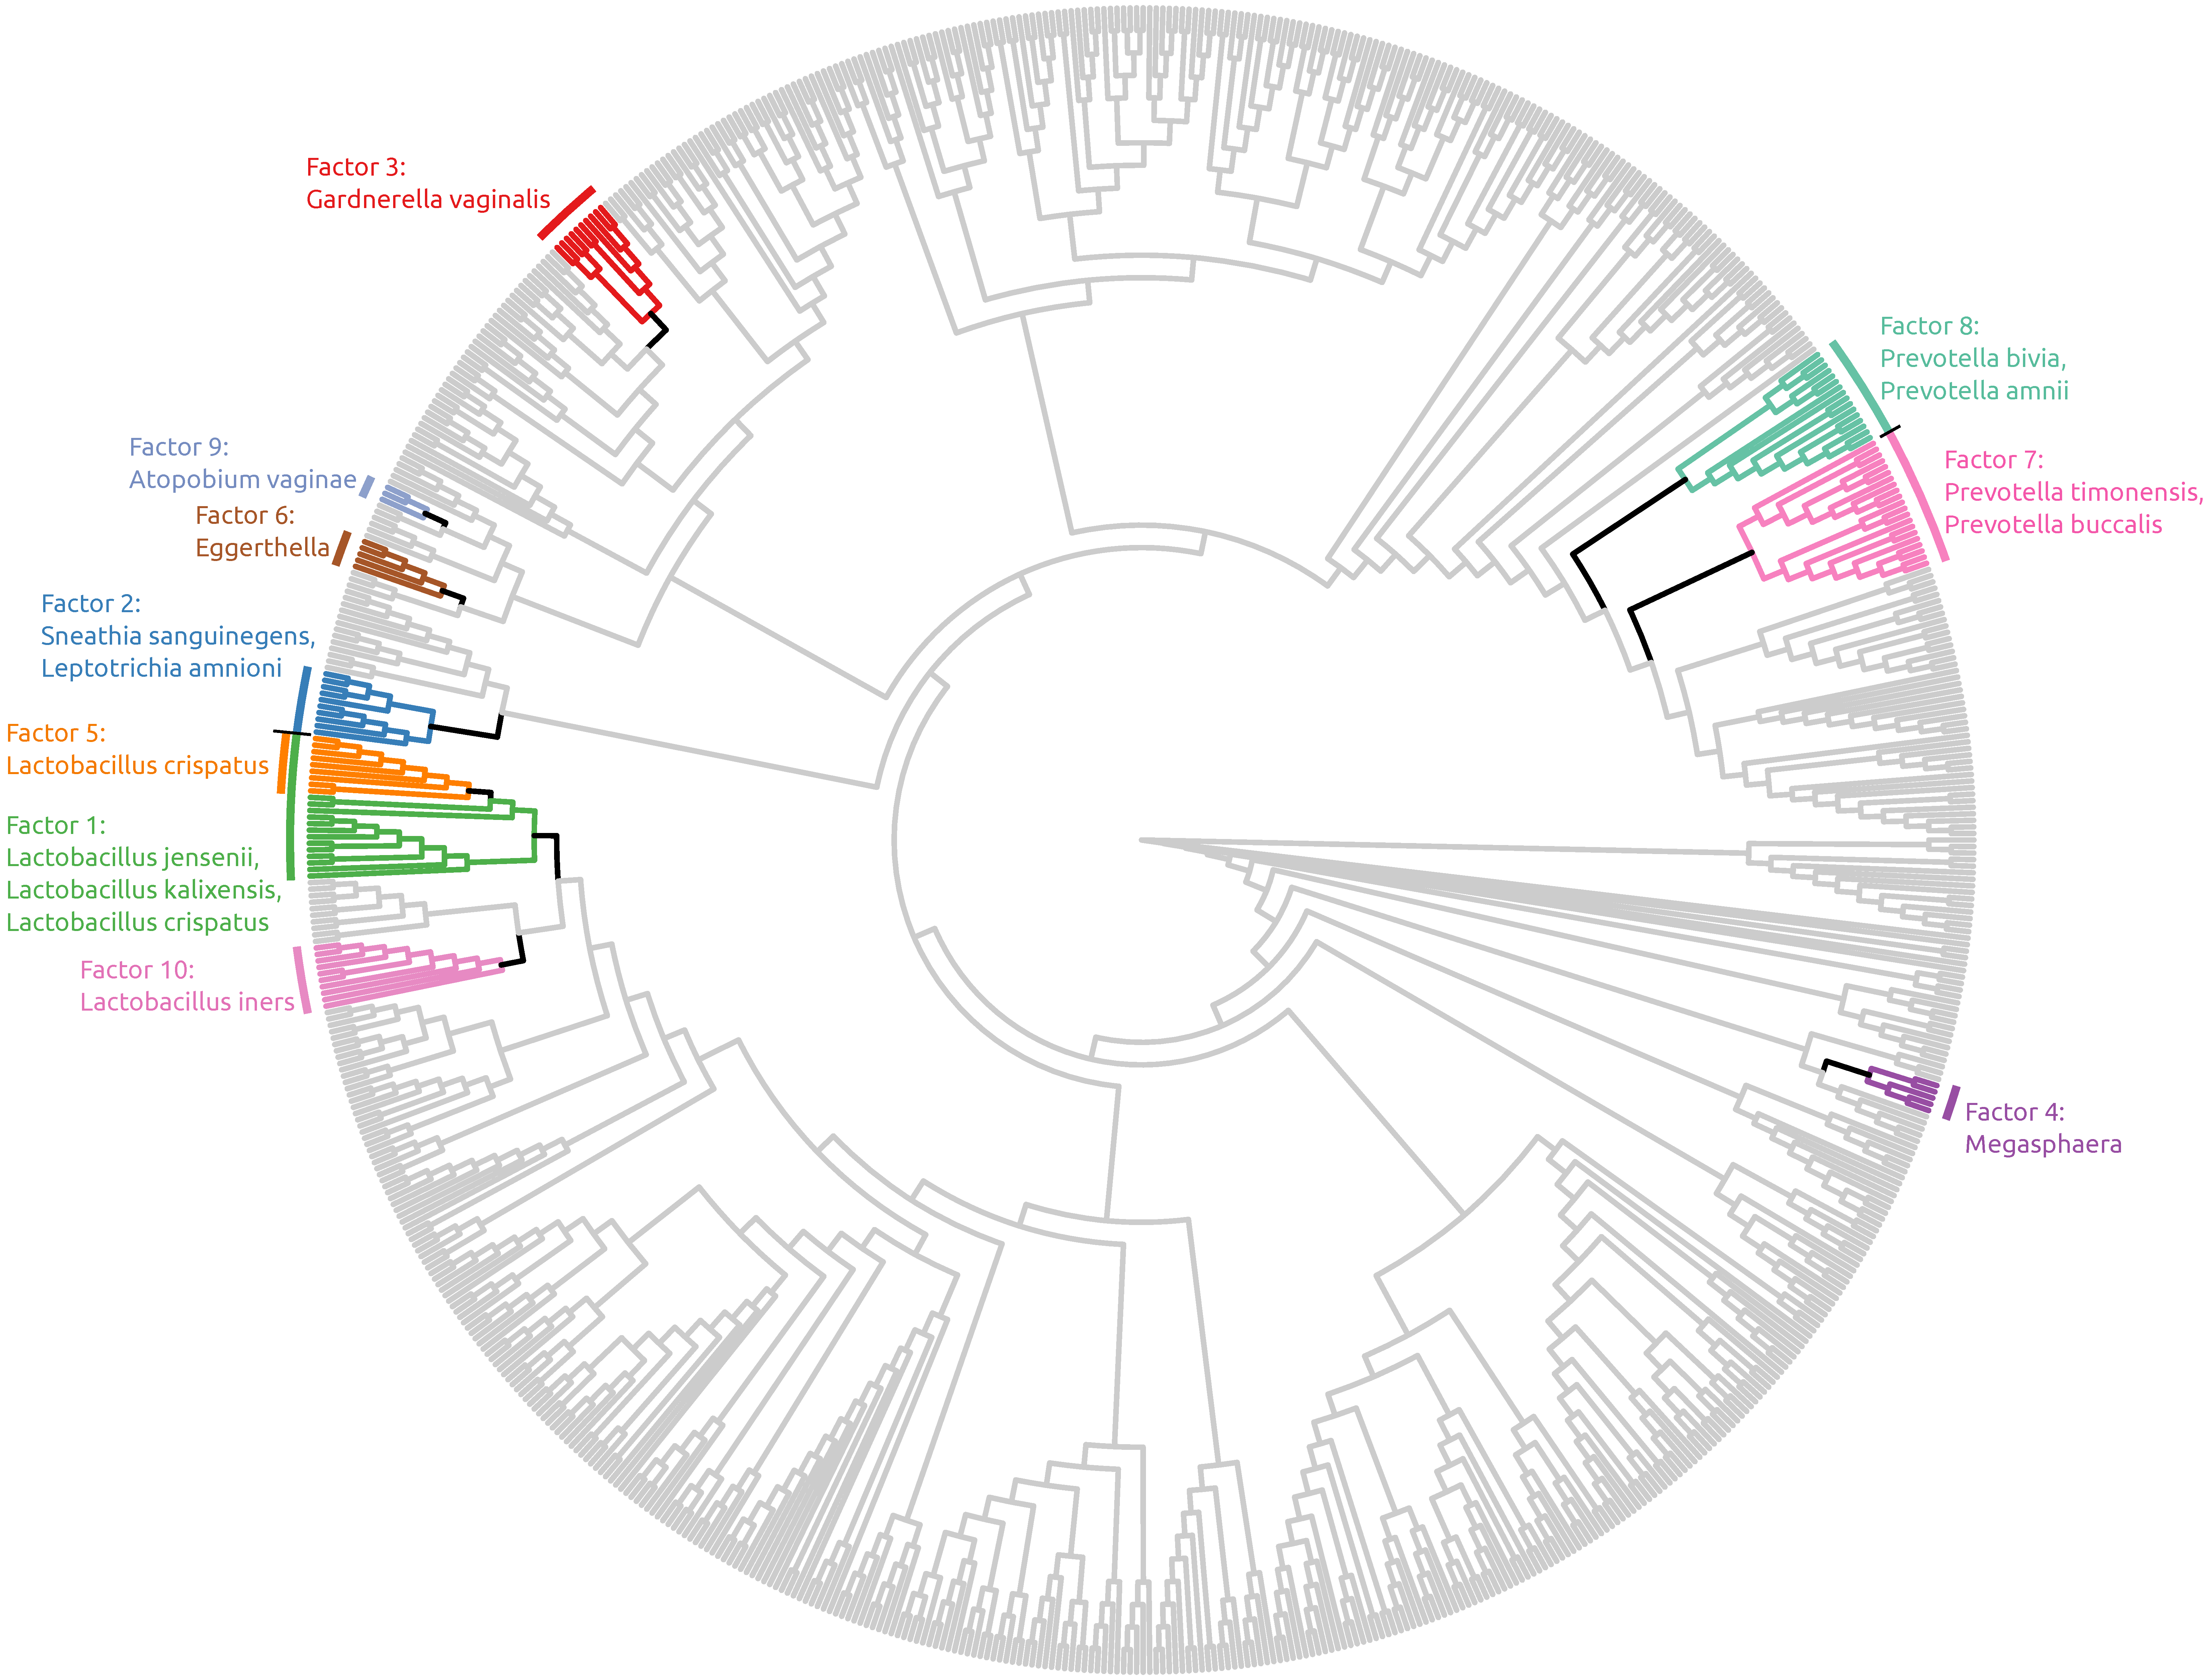
\includegraphics[width=\linewidth]{pdf/factors_tree.pdf}
    \caption[Visualization of the first ten factors of the \acs{BV} dataset]{
        \textbf{Visualization of the first ten factors of the \ac{BV} dataset.}
        Here, we show the first ten factors found by Placement-Factorization without taxon weighting on the \ac{BV} dataset.
        The black edges are the winning edges of each iteration, which split the tree into several subtrees.
        For simplicity, we only colored the clades leading away from the (arbitrarily placed) root,
        while leaving the paraphyletic ``remainder'' clade in gray.
        Note that factor 5 is nested in factor 1, that is, it further splits the branches within the first factor,
        thus separating \taxonname{Lactobacillus crispatus}
        from \taxonname{Lactobacillus jensenii} and \taxonname{Lactobacillus kalixensis}.
        See \tabref{tab:bv_phylofactor_clades} for a comparison of the clades separated by each factor
        to the factors found by the original Phylofactorization.
        Furthermore, see \figref{fig:pf_bv_place_ilr_ordination:sub:without_taxon_weighting} for an ordination
        of the first two factors, showing how these factors separate the samples in the dataset.
    }
    \label{fig:factors_tree}
\end{figure}

These outcomes show that our results are consistent with the existing Phylofactorization,
in that similar clades are split from the tree,
albeit with some variation in the order by which clades are selected. % in which factor/iteration.
The clades being split are also consistent with previous analyses of the dataset \cite{Srinivasan2012},
as all taxa found by the first ten factors of Placement-Factorization
were also found to be relevant in the context of \acl{BV} in \cite{Srinivasan2012}.
% However, our method as well as the \toolname{swarm}-based Phylofactorization did not
% except for the \toolname{vsearch}-based Phylofactorization, the
However, the \toolname{vsearch}-based Phylofactorization is the only evaluated variant
that split the \taxonname{Lactobacillus} clade in the first factor
and further \taxonname{Lactobacillus crispatus} from \taxonname{Lactobacillus iners} in the second factor.
The \toolname{swarm}-based variant and our Placement-Factorization without taxon weighting also identified these clades,
but not in the first two iterations.

% ------------------------------------------------
%     Visualization of the Objective Function
% ------------------------------------------------

\paragraph{Visualization of the Objective Function}
\label{sec:Factorization:sub:Evaluation:sub:BVDataset:par:VizObjective}

Above, we have compared Placement-Factorizaiton \emph{without} taxon weighting to the original Phylofactorization,
which currently does not support any taxon weighting schemes.
When using taxon weighting on the other hand,
Placement-Factorization also finds the two \taxonname{Lactobacillus} clades in the first two factors,
and is hence more consistent with existing analyses of the dataset.
However, due to small differences in the value of the objective function,
the winning edge of the first iteration
is chosen to be relatively basal in the tree, meaning that a large clade is factored out.
We observed a similar behavior with the \toolname{vsearch}-based Phylofactorization;
as can be seen by the long list of taxa of the first factor in \tabref{tab:bv_phylofactor_clades}.
In order to identify the provenance of this effect and to correctly interpret the factors,
we developed a novel visualization of the results:
In \figref{fig:pf_bv_place_tw_ovs}, we show the reference tree,
% In \figref{fig:pf_bv_place_tw_ovs} and in \figref{fig:pf_bv_place_no_tw_ovs}, we show the reference tree,
where each edge is colored by the value of the objective function at that edge.

\begin{figure}[btp!]
    \centering
    \includegraphics[width=\linewidth]{pdf/pf_bv_place_tw_ovs.pdf}
    \begin{subfigure}{0pt}
        \phantomcaption
        \label{fig:pf_bv_place_tw_ovs:sub:first}
    \end{subfigure}
    \begin{subfigure}{0pt}
        \phantomcaption
        \label{fig:pf_bv_place_tw_ovs:sub:second}
    \end{subfigure}
    \caption[Objective values of Placement-Factorization with taxon weighting of the \acs{BV} dataset]{
        \textbf{Objective values of Placement-Factorization with taxon weighting of the \ac{BV} dataset.}
        Here, we show the values of the objective function for each inner edge,
        for the first two factors found by Placement-Factorization \emph{with} taxon weights of the \ac{BV} dataset.
        The winning edge of each iteration is marked by a black arrow.
        See also \figref{fig:pf_bv_place_no_tw_ovs} for the version of this visualization \emph{without} taxon weights.
    }
    \label{fig:pf_bv_place_tw_ovs}
\end{figure}

This novel type of visualization helps to assess the uncertainty
involved in identifying the winning edge of a specific iteration:
The objective function of the first iteration in \figref{fig:pf_bv_place_tw_ovs:sub:first} for instance
yields high values for the path towards the \taxonname{Lactobacillus} clade, consistent with previous findings.
Random variability however leads to the first iteration splitting a larger clade
than expected when using taxon weighting, marked with an arrow.
% By observing the whole set taxa of this clade, it would not be obvious that this factor is mostly concerning
This obfuscates the fact that this factor is mostly concerning the \taxonname{Lactobacillus} clade,
and not so much the remaining taxa in that clade.
The clade includes many branches and taxa with a low value of the objective function (yellow branches),
% This indicates that these taxa are not relevant for this factor.
which are branches with low placement mass that do not contribute much to this factor.
There is however a path of comparably high values of the objective function (dark branches)
that leads down to the \taxonname{Lactobacillus} clade.
This indicates that there are several `good' candidate edges for distinguishing patients by their health status,
and that the smaller \taxonname{Lactobacillus} clade is the actual clade of interest in this factor.
The winning edge just happened to have a slightly higher value than other edges on this path.
The visualization thus aids interpretation of the factors,
helps to understand why a particular edge was chosen in an iteration,
and allows to identify the parts of a factored clade that are most relevant to the factor.

To address this issue of random variability, a proper statistical test of the significance of each winning edge
compared to the other edges evaluated in the iteration could be employed.
This is connected to the idea of \emph{confidence regions} of each factor on the tree,
as presented in \cite{Washburne2019}, which we discuss later.
%, but leave this as future work.
Note that in the second iteration in \figref{fig:pf_bv_place_tw_ovs:sub:second},
the tree clearly shows the distinction between the two relevant clades of \taxonname{Lactobacillus} again,
consistent with previous findings.
Hence, even with the first factor splitting a relatively large clade,
the second factor correctly identified the relevant edges within this large clade.

Lastly, we show the same type of visualization for Placement-Factorization \emph{without} taxon weighting
in \figref{fig:pf_bv_place_no_tw_ovs}.
The figure hence again corresponds to the analyses presented above
in \tabref{tab:bv_phylofactor_clades} and \figref{fig:factors_tree}.

\begin{figure}[!htb]
    \centering
     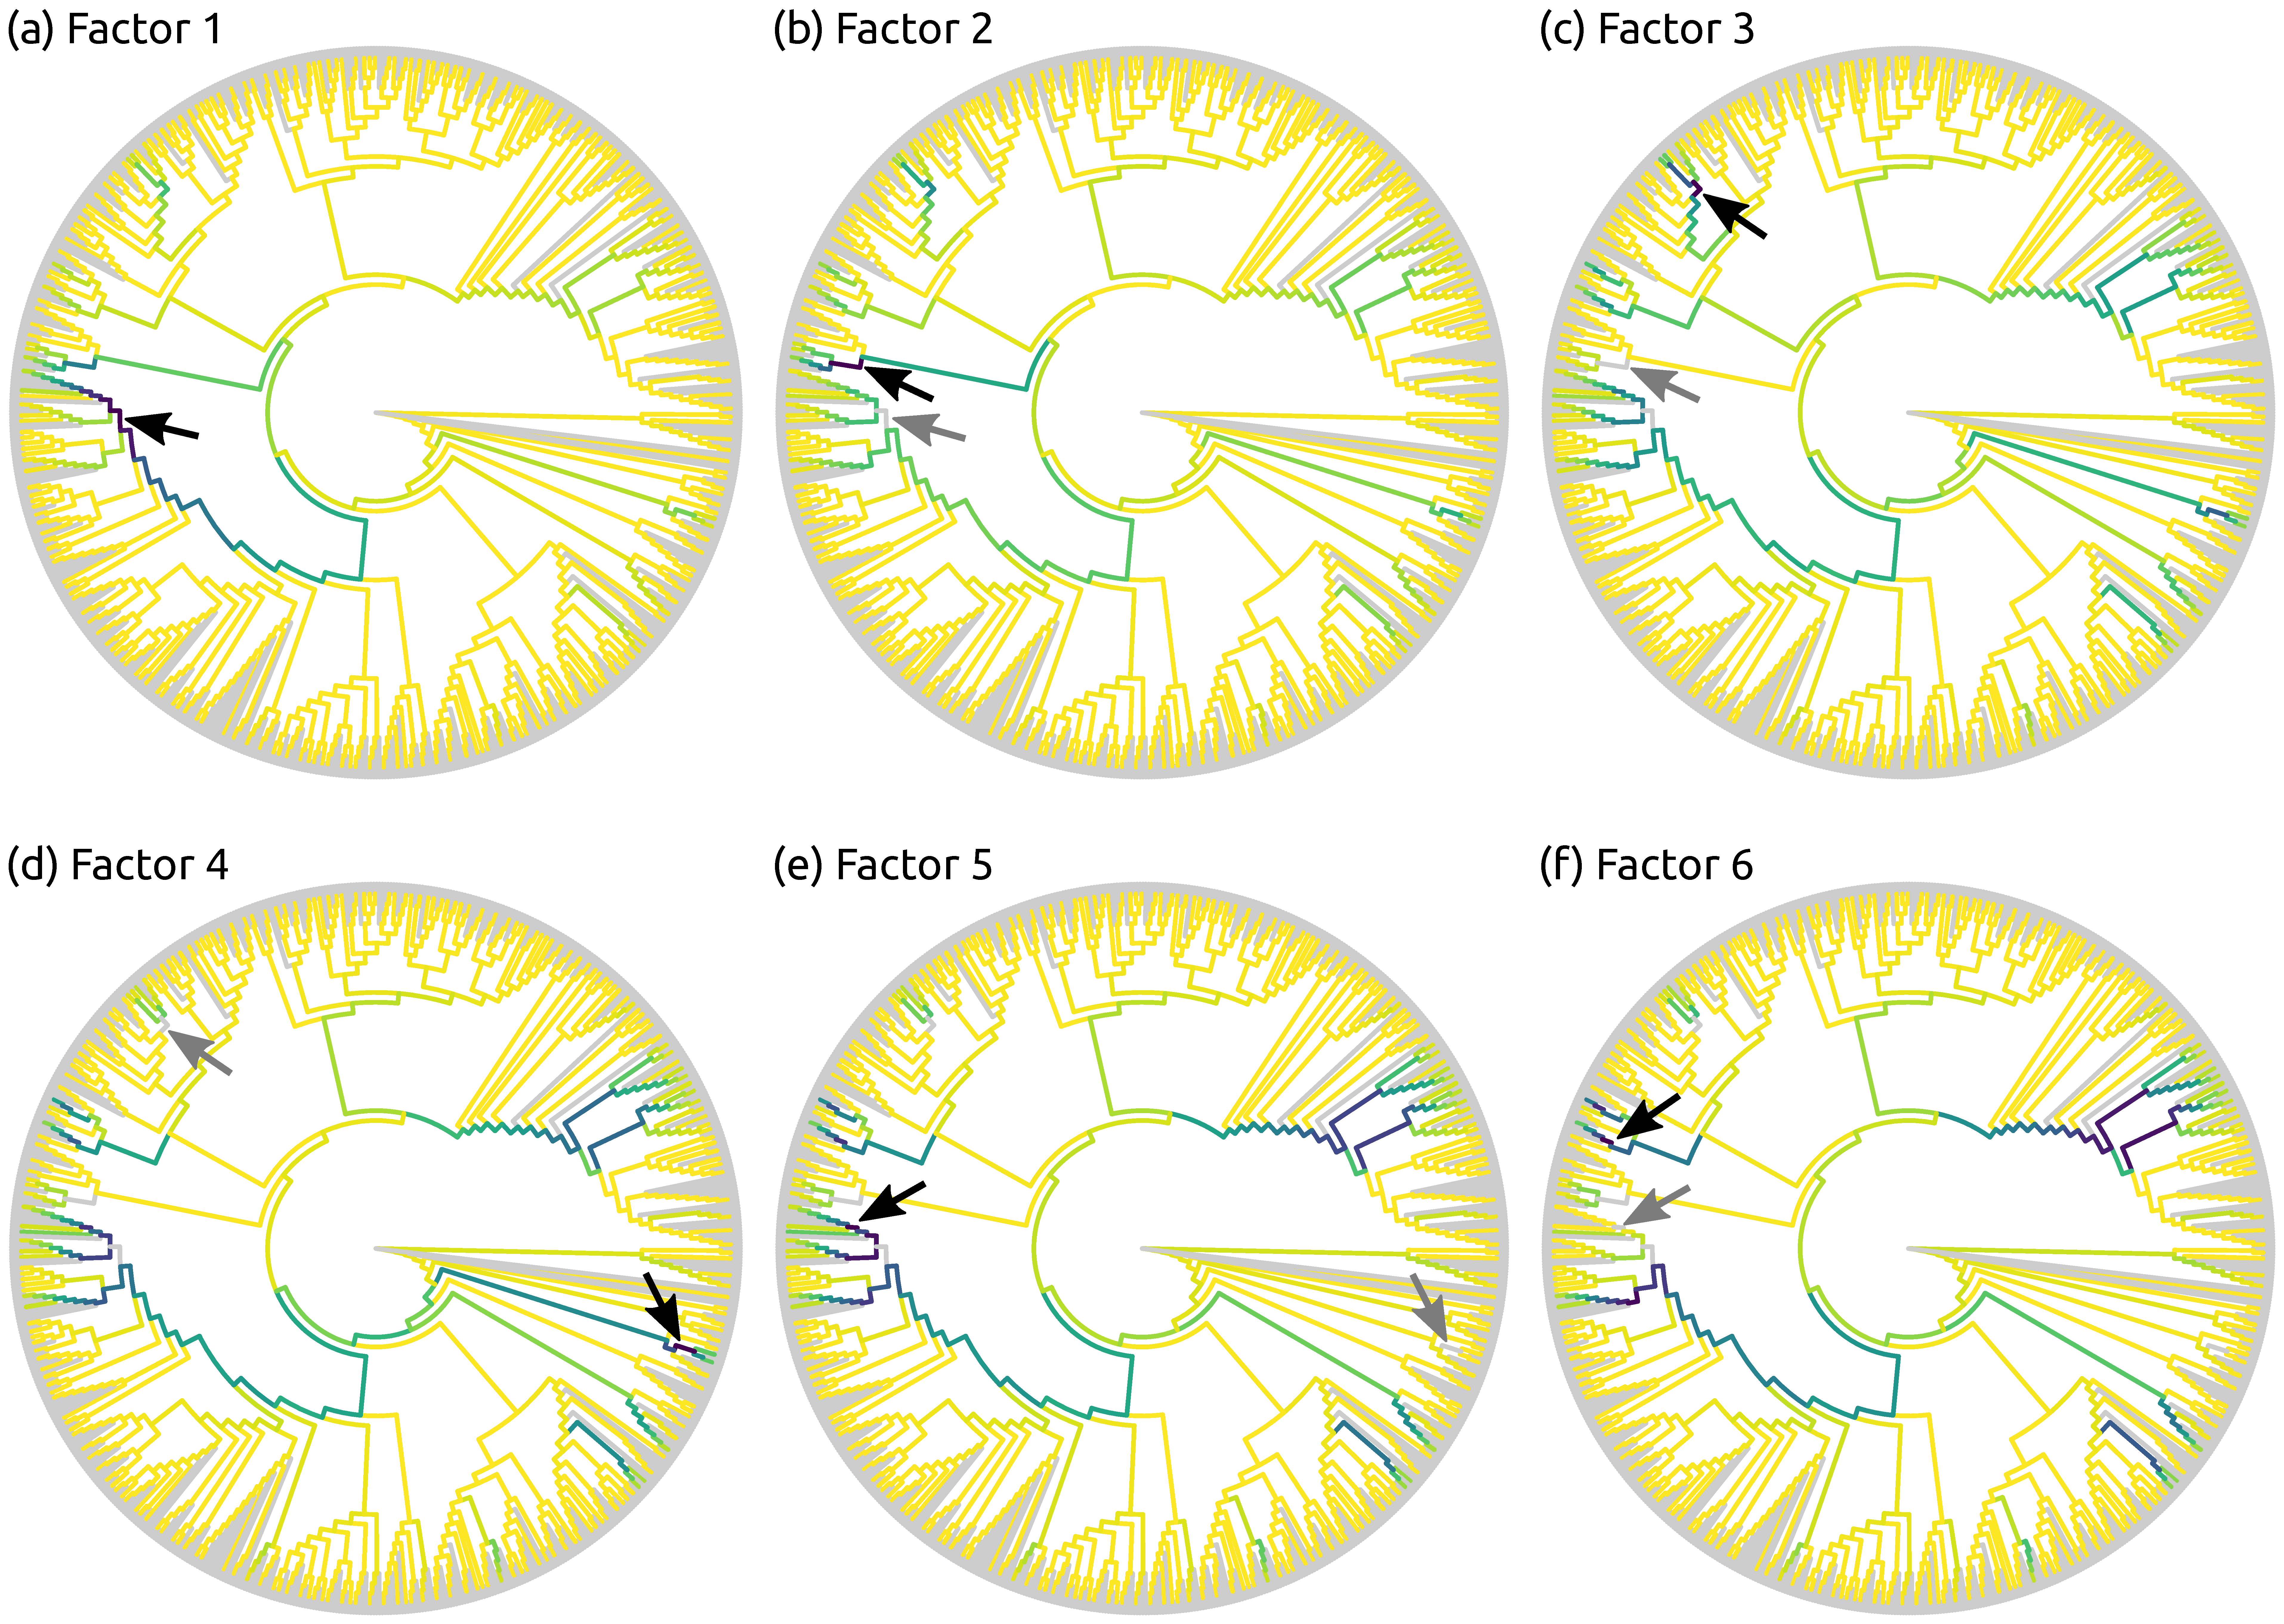
\includegraphics[width=\linewidth]{pdf/pf_bv_place_no_tw_ovs.pdf}
    \begin{subfigure}{0pt}
        \phantomcaption
        \label{fig:pf_bv_place_no_tw_ovs:sub:factor_1}
    \end{subfigure}
    \begin{subfigure}{0pt}
        \phantomcaption
        \label{fig:pf_bv_place_no_tw_ovs:sub:factor_2}
    \end{subfigure}
    \begin{subfigure}{0pt}
        \phantomcaption
        \label{fig:pf_bv_place_no_tw_ovs:sub:factor_3}
    \end{subfigure}
    \begin{subfigure}{0pt}
        \phantomcaption
        \label{fig:pf_bv_place_no_tw_ovs:sub:factor_4}
    \end{subfigure}
    \begin{subfigure}{0pt}
        \phantomcaption
        \label{fig:pf_bv_place_no_tw_ovs:sub:factor_5}
    \end{subfigure}
    \begin{subfigure}{0pt}
        \phantomcaption
        \label{fig:pf_bv_place_no_tw_ovs:sub:factor_6}
    \end{subfigure}
    \caption[Objective function values for the first six factors of the \acs{BV} dataset without taxon weighting]{
        \textbf{Objective function values for the first six factors of the \ac{BV} dataset without taxon weighting.}
%         In each iteration of Phylofactorization and Placement-Factorization, the objective function is evaluated
%         for each edge of the tree (except for edges that were winning previous iterations).
        The figure visualizes the value of the objective function for the first six iterations of
        Placement-Factorization of the \ac{BV} dataset, \emph{without} taxon weighting.
        Darker edges represent higher values;
        the highest value of each iteration (the winning edge) is marked with a black arrow.
        Gray arrows further mark the winning edge of the respective previous iteration,
        which allows to examine the effect of ``factoring out'' an edge.
%         The clades of the winning edges shown here can also be seen in \figref{fig:factors_tree},
%         and are listed in \tabref{tab:bv_phylofactor_clades}.
        See also \figref{fig:pf_bv_place_tw_ovs} for the according visualization \emph{with} taxon weights.
%         Some of the edges with high OFVs in \subref{fig:pf_bv_place_no_tw_ovs:sub:factor_6} are subsequently
%         picked in later iterations of the factorization, as can be seen in \figref{fig:factors_tree}.
    }
    \label{fig:pf_bv_place_no_tw_ovs}
\end{figure}

Apart from the guidance for interpreting the factors, the figure also reveals another aspect of Phylofactorization:
By comparing the values of the objective function on the tree between subsequent iterations,
one can observe the effect of ``factoring out'' an edge.
Due to the nature of comparing the two sides induced by an edge,
high values of the objective function usually propagate across several connected edges,
e.\,g., the region of dark branches around the marked edge in \figref{fig:pf_bv_place_no_tw_ovs:sub:factor_1}.
Once a factor has been split from the tree, the values for the whole path drop,
which can be seen by comparing \figref{fig:pf_bv_place_no_tw_ovs:sub:factor_1}
and \subref{fig:pf_bv_place_no_tw_ovs:sub:factor_2},
where the region around the gray arrow has much lower values of the objective function.
This behavior can consistently be observed in the other subfigures as well.
% This corresponds to the effect of
% which allows to examine the effect of
% The gray arrows in \figref{fig:pf_bv_place_no_tw_ovs} mark the winning edge of the respective previous iteration.
The figure hence shows that factoring out an edge actually removes nested depenendices between factors, as expected.

% ------------------------------------------------
%     Further Assessment
% ------------------------------------------------

\paragraph{Further Assessment}
\label{sec:Factorization:sub:Evaluation:sub:BVDataset:par:FurtherAssessment}

To further assess how the samples are split by individual factors,
we used the balances at each iteration/factor as an ordination of the data, as suggested in \citeay{Washburne2017a},
which we show in \figref{fig:pf_bv_place_ilr_ordination}.
These plots reveal that the splitting into healthy vs.~diseased patients works both with and without taxon weighting,
albeit the differences in the respective plot shapes are pronounced.

\begin{figure}[!htb]
    \centering
     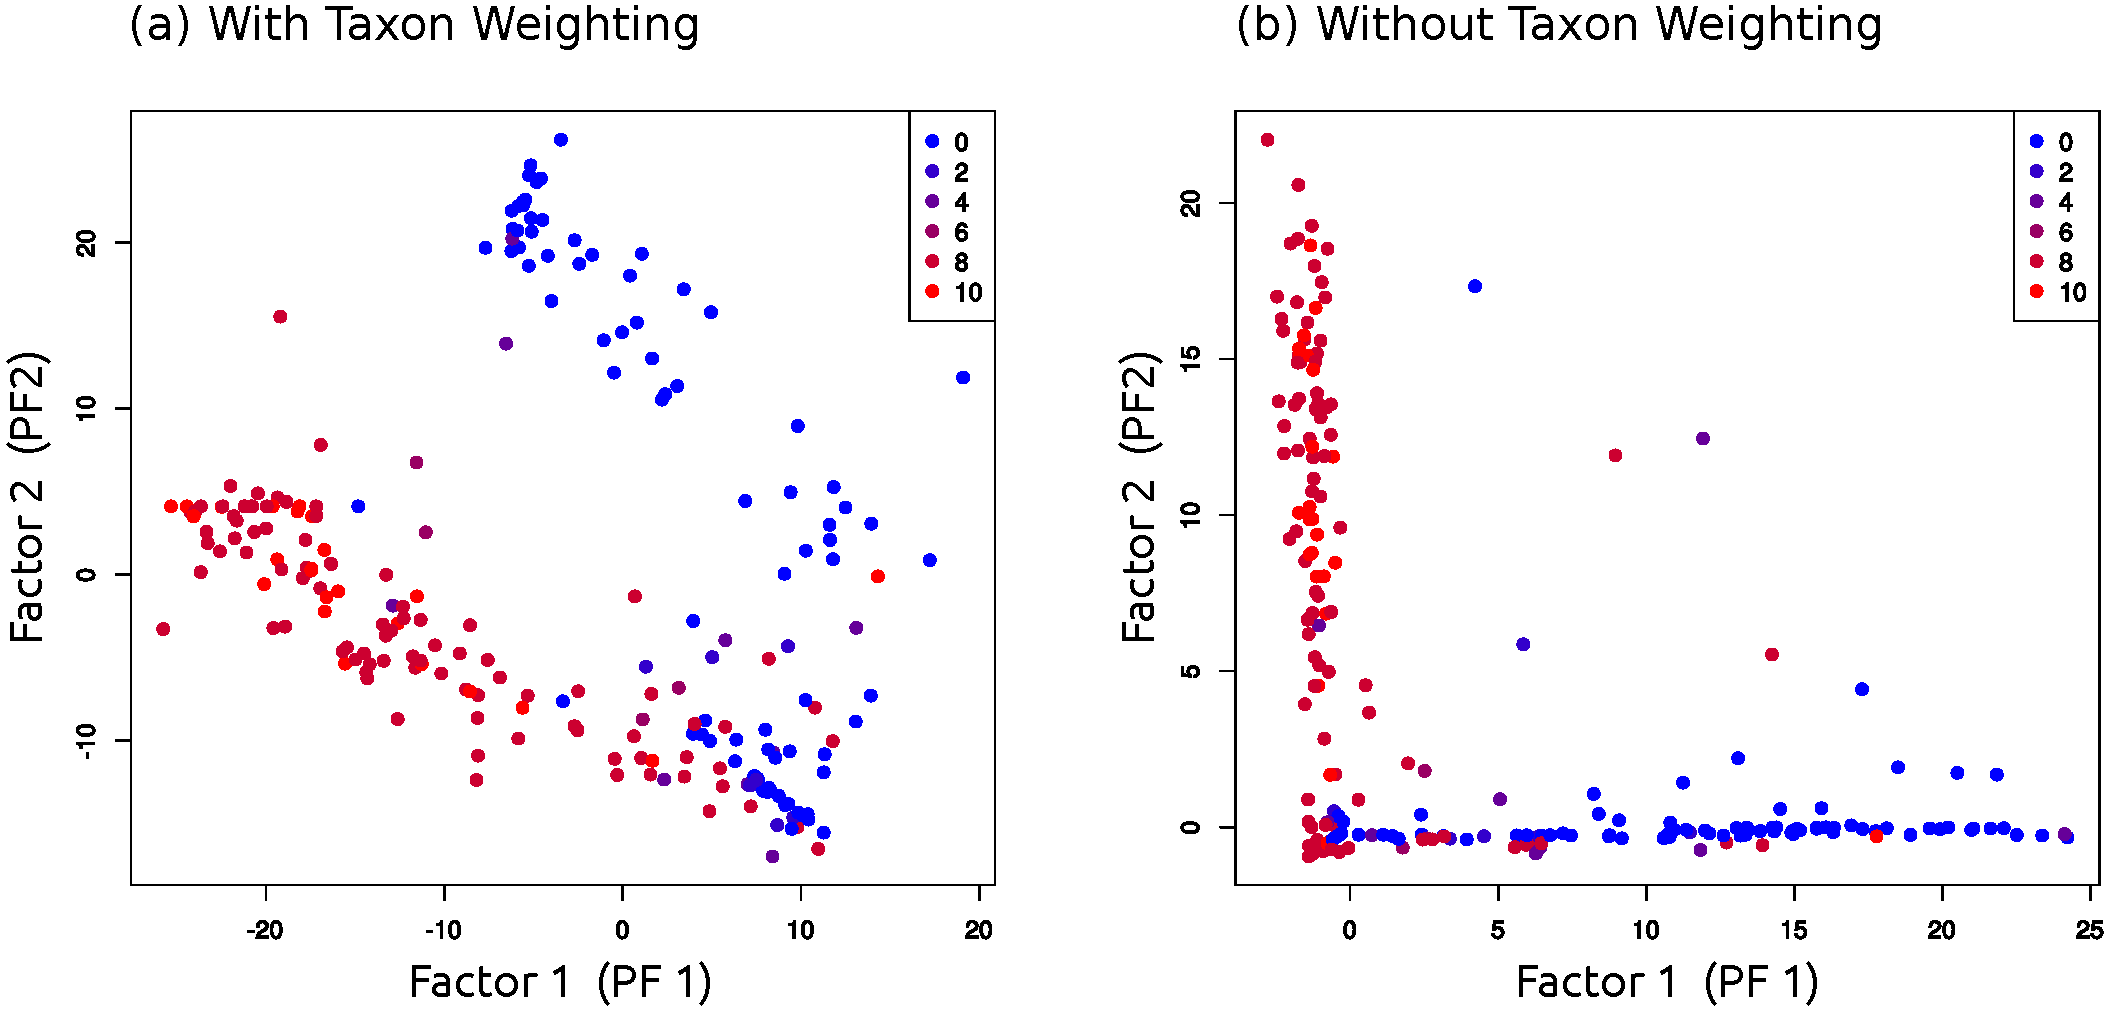
\includegraphics[width=\linewidth]{pdf/pf_bv_place_ilr_ordination.pdf}
    \begin{subfigure}{0pt}
        \phantomcaption
        \label{fig:pf_bv_place_ilr_ordination:sub:with_taxon_weighting}
    \end{subfigure}
    \begin{subfigure}{0pt}
        \phantomcaption
        \label{fig:pf_bv_place_ilr_ordination:sub:without_taxon_weighting}
    \end{subfigure}
    \caption[Ordination of the first two factors of the \acs{BV} dataset]{
        \textbf{Ordination of the first two factors of the \ac{BV} dataset.}
        The figure shows ordination-visualization plots of the ILR coordinates (balances) of the first two factors
        found by Placement-Factorization of the \ac{BV} dataset,
        \subref{fig:pf_bv_place_ilr_ordination:sub:with_taxon_weighting} with and
        \subref{fig:pf_bv_place_ilr_ordination:sub:without_taxon_weighting} without taxon weighting.
        That is, the axes correspond to the splits induced by the first two factors,
        while values along the axes are the balances of each sample calculated on the sets of edges of each split.
        Samples are again colored by their Nugent score, with \num{0} being the healthy patients,
        and \num{10} being the patients with severe \ac{BV}.
        See \figref{fig:pf_bv_place_tw_ovs} for the (winning) edges that correspond to the axes
        in \subref{fig:pf_bv_place_ilr_ordination:sub:with_taxon_weighting} (with taxon weighting),
        and see \figref{fig:factors_tree} and \tabref{tab:bv_phylofactor_clades}
        for the edges corresponding to the axes in \subref{fig:pf_bv_place_ilr_ordination:sub:without_taxon_weighting}
        (without taxon weighting).
%         explain signs and magnitudes along the axes: denominator, small clades
%         auto const balances = mass_balance( data, p_indices, s_indices );
    }
    \label{fig:pf_bv_place_ilr_ordination}
\end{figure}

On the one hand, Placement-Factorization \emph{with} taxon weighting
in \figref{fig:pf_bv_place_ilr_ordination:sub:with_taxon_weighting}
is highly similar to PCA on the balances
as shown in \figref{fig:bv_place_edge_balances_pca_scatter:sub:with_taxon_weighting},
despite the fact that PCA does not take the meta-data into account.
We suspect that is is due to the nature of the dataset,
were the abundances in the \taxonname{Lactobacillus} clade almost solely dictate the health status of each individual,
and roughly half the samples belong to either the healthy or the sick group of patients.
Hence, the \taxonname{Lactobacillus} clade naturally is a major driver of differences between samples,
and is thus identified by PCA as the most important component/axis.
%         As shown in \figref{fig:pf_bv_place_tw_ovs}, the first factor of the taxon-weighted Placement-Factorization
%         splits a rather large clade from the tree.
%         Hence, there are

On the other hand, Placement-Factorization \emph{without} taxon weighting
in \figref{fig:pf_bv_place_ilr_ordination:sub:without_taxon_weighting} yields an ordination
that separates healthy from sick patients in the first factor,
and further splits the sick patients in the second factor.
The reason for this can be seen in the clades that each factor splits away from the tree,
as shown in \figref{fig:factors_tree}:
The first factor separates part of the \taxonname{Lactobacillus} clades,
which explains why it distinguishes samples based on heath status.
The second factor separates a clade containing \taxonname{Sneathia sanguinegens} and \taxonname{Leptotrichia amnioni},
which is an important clade among several clades that are associated with \ac{BV} \cite{Srinivasan2012}.
This can also be seen in \figref{fig:heat_tree},
where the healthy patients with low Nugent score
almost exclusively exhibit high abundances of \taxonname{Lactobacillus},
while the diseased patients with high Nugent score show abundances in several clades all over the tree.

\figref{fig:pf_bv_place_ilr_ordination} hence serves as a caveat for Phylofactorization and Placement-Factori\-zation,
and as an example of the limitations of this type of plot.
These plots were suggested in \citeay{Washburne2017a} as an additional way of depicting
how the factors separate samples according to meta-data features, see their Figure~5(a).
Note that such visualizations can only reasonably visualize the first two or three factors,
which is why they are now discontinued in the original Phylofactorization
(pers.~comm. with A.~Washburne on 2019-01-16).

In the case of the \ac{BV} dataset, %\subref{fig:pf_bv_place_ilr_ordination:sub:without_taxon_weighting},
two axes/factors are sufficient to separate the samples by Nugent score.
% that is, to separate healthy from diseased patients,
% but they do not explain the multitude of clades that are associated with \ac{BV}.
That is, the \ac{BV} dataset does indeed have two important features concerning the \emph{healthy} patients,
namely the \taxonname{Lactobacillus} clade, and the further distinction
into \taxonname{Lactobacillus crispatus} and \taxonname{Lactobacillus iners}.
However, as discussed above and visible in \figref{fig:heat_tree},
the \emph{diseased} patients exhibit high abundances in a multitude of other clades,
which cannot be expressed by just two or three factors.

It is hence crucial to compute all significant factors---otherwise,
important aspects of the data get lost and results are incomplete.
We also developed a novel way of visualizing the balances of further factors,
as for example shown later for the \ac{HMP} dataset in \figref{fig:hmp_pf_of_600_factor_ordination},
which alleviates this issue.

% Although for the \ac{BV} dataset, two factors suffice to show the major features,
%   As scatter plots of balances can only reasonably reveal the first two or three factors,
% \figref{fig:pf_bv_place_ilr_ordination} hence serves as a caveat for the limitations of this type of visualization:

% We later show a novel way for visualizing balances in the \ac{HMP} dataset that can help to understand
% the balances of all factors in \secref{sec:Factorization:sub:Evaluation:sub:HMPDataset:par:FullDataset}.
%In the absence of additional meta-data other than health status of the \ac{BV} dataset however,
%these novel visualization would not yield any further helpful information here, which is why we introduce them later.

% ----------------------------------------------------------------------------------------------------------------------
%     Tara Dataset
% ----------------------------------------------------------------------------------------------------------------------

% \subsubsection*{Tara Oceans dataset}
% \label{sec:Results:sub:Phylofactor:sub:TaraDataset}

% Nothing nice to report yet... Will need more time for this.

% ----------------------------------------------------------------------------------------------------------------------
%     HMP Dataset
% ----------------------------------------------------------------------------------------------------------------------

\subsection{Oral/Fecal Subset of the HMP dataset}
\label{ch:Factorization:sec:Evaluation:sub:OralFecalHMPDataset}

We here show the analysis of a subset of the \acf{HMP} dataset \cite{Huttenhower2012,Methe2012},
in order to compare Placement-Factorization to findings of the original Phylofactorization
on a similar dataset \cite{Washburne2017a}.
See \appref{supp:sec:DetailsEmpiricalDatasets:sub:HMP} for details on the dataset and its preprocessing.

The original publication of Phylofactorization used a dataset comprising oral and fecal samples from the human microbiome
as one of their case studies \cite{Caporaso2011}, see Figure~4 and Supplementary Figures S3--S8 of \citeay{Washburne2017a}.
For our comparison, we selected a suitable subset of the \ac{HMP} dataset: % \cite{Huttenhower2012,Methe2012}:
In particular, we selected all \num{600} stool samples of the dataset,
as well as \num{600} randomly chosen samples from the mouth region,
that is, from the samples labeled ``Mouth (back)'' and ``Mouth (front)'' in \tabref{tab:hmp_data_overview}.
We again used the placement of these samples on the unconstrained \taxonname{Bacteria} tree
of our \acf{PhAT} method to conduct Placement-Factorization.
The tree contains \num{1 914} taxa, as explained in \secref{ch:AutomaticTrees:sec:Evaluation}.
We henceforth assume that the oral/fecal dataset of \citeay{Caporaso2011}
and our oral/fecal subset of the \ac{HMP} dataset exhibit comparable sequence compositions.
Furthermore, as the tree used for Phylofactorization in \citeay{Washburne2017a} is based on the OTUs of the sequences,
it only contains taxa that are sufficiently abundant in the input.
It thus differs from the more general \taxonname{Bacteria} reference tree used for our evaluation here.
Therefore, we had to map the taxa found by Phylofactorization
to the underlying \toolname{Silva} taxonomy \cite{Quast2013,Yilmaz2014} that was used for constructing our reference tree.
% To this end, we mapped the taxa of the latter to the \toolname{Silva} taxonomy \cite{Quast2013,Yilmaz2014}
% that was used for constructing the reference tree shown here \cite{Czech2018}.

% ------------------------------------------------
%     Comparison to Phylofactorization
% ------------------------------------------------

\paragraph{Comparison to Phylofactorization}
\label{sec:Factorization:sub:Evaluation:sub:OralFecalHMPDataset:par:Comparison}

Despite these differences, Placement-Factorization yielded factors that are similar to the ones found by Phylofactorization.
We again used Placement-Factorization \emph{with} and \emph{without} taxon weighting,
and compare the taxa identified by the first \num{10} factors
to the the first \num{10} factors found in the original oral/fecal dataset with Phylofactorization \cite{Washburne2017a}.
We visualized the clades found by all three variants in \figref{fig:multi_factors_tree}.

\afterpage{
\begin{landscape}
\begin{figure}[!htbp]
    \centering
     \includegraphics[width=0.828\linewidth]{pdf/multi_factors_tree.pdf}
    \caption[Comparison of factors found in the oral/fecal subset of the \acs{HMP} dataset]{
        \textbf{Comparison of factors found in the oral/fecal subset of the \ac{HMP} dataset.}
        Here, we compare the first \num{10} factors found by Placement-Factorization with and without taxon weighting
        on an oral/fecal subset of the \ac{HMP} dataset
        to the first \num{10} factors found by Phylofactorization on their oral/fecal test dataset \cite{Caporaso2011,Washburne2017a}.
        The clades of the tree are colored so that green, blue, and red mark branches that only appear in one of the variants,
%         (Placement-Factorization with and without taxon weighting, and Phylofactorization, respectively),
        cyan, yellow, and purple for branches that occurred in two variants,
        and dark gray for branches that were found by all three variants.
        For simplicity, we here neglect the order and nesting of factors.
        That is, if a branch is part of the non-root side of any one of the first ten factors, it is colorized here.
%         without considering in which iteration it was found.
    }
    \label{fig:multi_factors_tree}
\end{figure}
\end{landscape}
} %afterpage

For simplicity, we only compare the clades on the non-root side of the (arbitrarily rooted) reference tree;
the paraphyletic ``remainder'' clade is not taken into account.
Furthermore, we do not consider the order of the factors here.
Similar to the findings of the \ac{BV} dataset above,
Placement-Factorization \emph{with} taxon weighting yielded larger clades than \emph{without} taxon weighting,
which again yielded larger clades than the OTU-based Phylofactorization.
The latter is a consequence of the OTU tree containing fewer taxa than our broad \taxonname{Bacteria} tree.
We found that 84\% of the taxa identified by Phylofactorization were also part of the factors of our variants,
with the major difference being a set of \taxonname{Proteobacteria}
that were part of the split in the first factor of Phylofactorization \cite{Washburne2017a}, but not by our variants.
This is most likely an artifact of the differing trees being used in the factorization.
Furthermore, 95\% of the taxa found by Placement-Factorization \emph{without} taxon weighting
were also part of the clades \emph{with} taxon weighting.

In particular, the larger clades found by variant with taxon weights
are shown as green edges in \figref{fig:multi_factors_tree}.
% finds larger clades than the other two.
% We already observed a similar behavior with the \ac{BV} dataset. %, as explained in \figref{fig:pf_bv_place_tw_ovs}.
The values of the objective function however indicate that the focus of the factor is in fact much smaller
and more in agreement with the other two variants compared here.
Again, this behavior is similar to the \ac{BV} data with taxon weighting;
see \figref{fig:pf_bv_place_tw_ovs} for details.
Furthermore, Phylofactorization found several small clades and single branches,
which are shown as red edges in \figref{fig:multi_factors_tree}.
% Furthermore, the several small clades and single branches found by Phylofactorization (red edges in \figref{fig:multi_factors_tree})
These branches are part of the \taxonname{Actinobacteria} as well as the \mbox{\taxonname{Alpha-},} \mbox{\taxonname{Beta-},}
\mbox{\taxonname{Gamma-},} and \taxonname{Deltaproteobacteria}, and are actually all part of the first factor.
They are marked with asterisks (*) in \figref{fig:multi_factors_tree}.
Due to their OTU tree only having few \taxonname{Proteobacteria},
these were monophyletic in their tree \cite{Washburne2017a}.
They are polyphyletic here, as our tree has more reference taxa from that group.
%a mismatching topology between the original OTU tree of the oral/fecal dataset of \cite{Washburne2017a} and our reference tree shown here.

Most of the remaining factors found by Phylofactorization are part of the gray branches
of the two large clades in \figref{fig:multi_factors_tree},
which are the clades that were found by all three variants.
% that were not picked by our variants.
Similarly, our variants found many nested factors (factors that further split a factor of a previous iteration):
The two large clades are in fact split into seven nested clades by both variants,
with the remaining three factors spread across the rest of the tree
(e.\,g., the green and blue branches of \figref{fig:multi_factors_tree}).
% We suspect that this is due to
% Lastly, note the gray branches, which mark clades that were found by all three variants:
In particular, the \taxonname{Prevotellaceae} and parts of the \taxonname{Firmicutes}
were described in \citeay{Washburne2017a} as important clades for the distinction between oral and fecal samples,
all of which were found by all three variants here.

% Most of the factors found by the three variants agree with each other,
% however with differences in the size of the clades.
% Despite the differences in the factors between Placement-Factorization and the original Phylofactorization,
% the clades found by our variants are well suited for separating oral from fecal samples,

In total, despite the mismatching trees, most of the found clades agree in all three variants,
with their disagreement mostly concerning the clade sizes.
More importantly, despite their differences,
all variants produce factors that are well suited for separating oral from fecal samples,
as further shown in the next section below. %later in \figref{fig:hmp_pf_of_600_factor_ordination}.

The actual differences in taxa (such as the \taxonname{Proteobacteria} not found by our variants)
serve as a caveat for the importance of the underlying reference tree:
Differences in topology will inevitably be reflected in different factors,
which might in turn suggest a different interpretation of results.
In an ideal world with a known phylogeny of all of life, alternative OTU clusterings and alternative trees
would simply collapse nodes at different depths (pers.~comm. with A.~Washburne on 2019-03-01).
Unfortunately, real world data, and particularly different OTU clustering methods and tree inference methods,
will yield discordant trees.
The influence of uncertainty in the phylogeny is further discussed in \citeay{Washburne2019}.

% no vs tw 0.954954954955
% tw vs no 0.649572649573
% no vs pf 0.418918918919
% pf vs no 0.8410041841
% tw vs pf 0.273504273504
% pf vs tw 0.845188284519

% ------------------------------------------------
%     Factor Ordination
% ------------------------------------------------

\paragraph{Factor Ordination}
\label{sec:Factorization:sub:Evaluation:sub:OralFecalHMPDataset:par:Ordination}

Next, we investigated how well the factors found by Placement-Factorization separate oral from fecal samples.
To this end, we again employed the balances of the winning edge of each factor for an ordination visualization \cite{Washburne2017a},
which we show in \figref{fig:hmp_pf_of_600_factor_ordination:sub:2d_with_taxon_weighting}
and \subref{fig:hmp_pf_of_600_factor_ordination:sub:2d_without_taxon_weighting}.
The ordination clearly separates the samples, both with and without taxon weighting.
Again, ordination scatter plots can only reveal up to three dimensions/factors.
In order to evaluate the separation of samples at later factors,
we use a visualization of the factor balances, which we call \emph{balance swarm plots},
and which are similar to the per-factor ordination plots used in \citeay{Washburne2019}.
These plots can show the ordination of arbitrarily many factors at the same time,
as shown in \figref{fig:hmp_pf_of_600_factor_ordination:sub:10d_with_taxon_weighting}
and \subref{fig:hmp_pf_of_600_factor_ordination:sub:10d_without_taxon_weighting}.

\begin{figure}[!htbp]
    \centering
     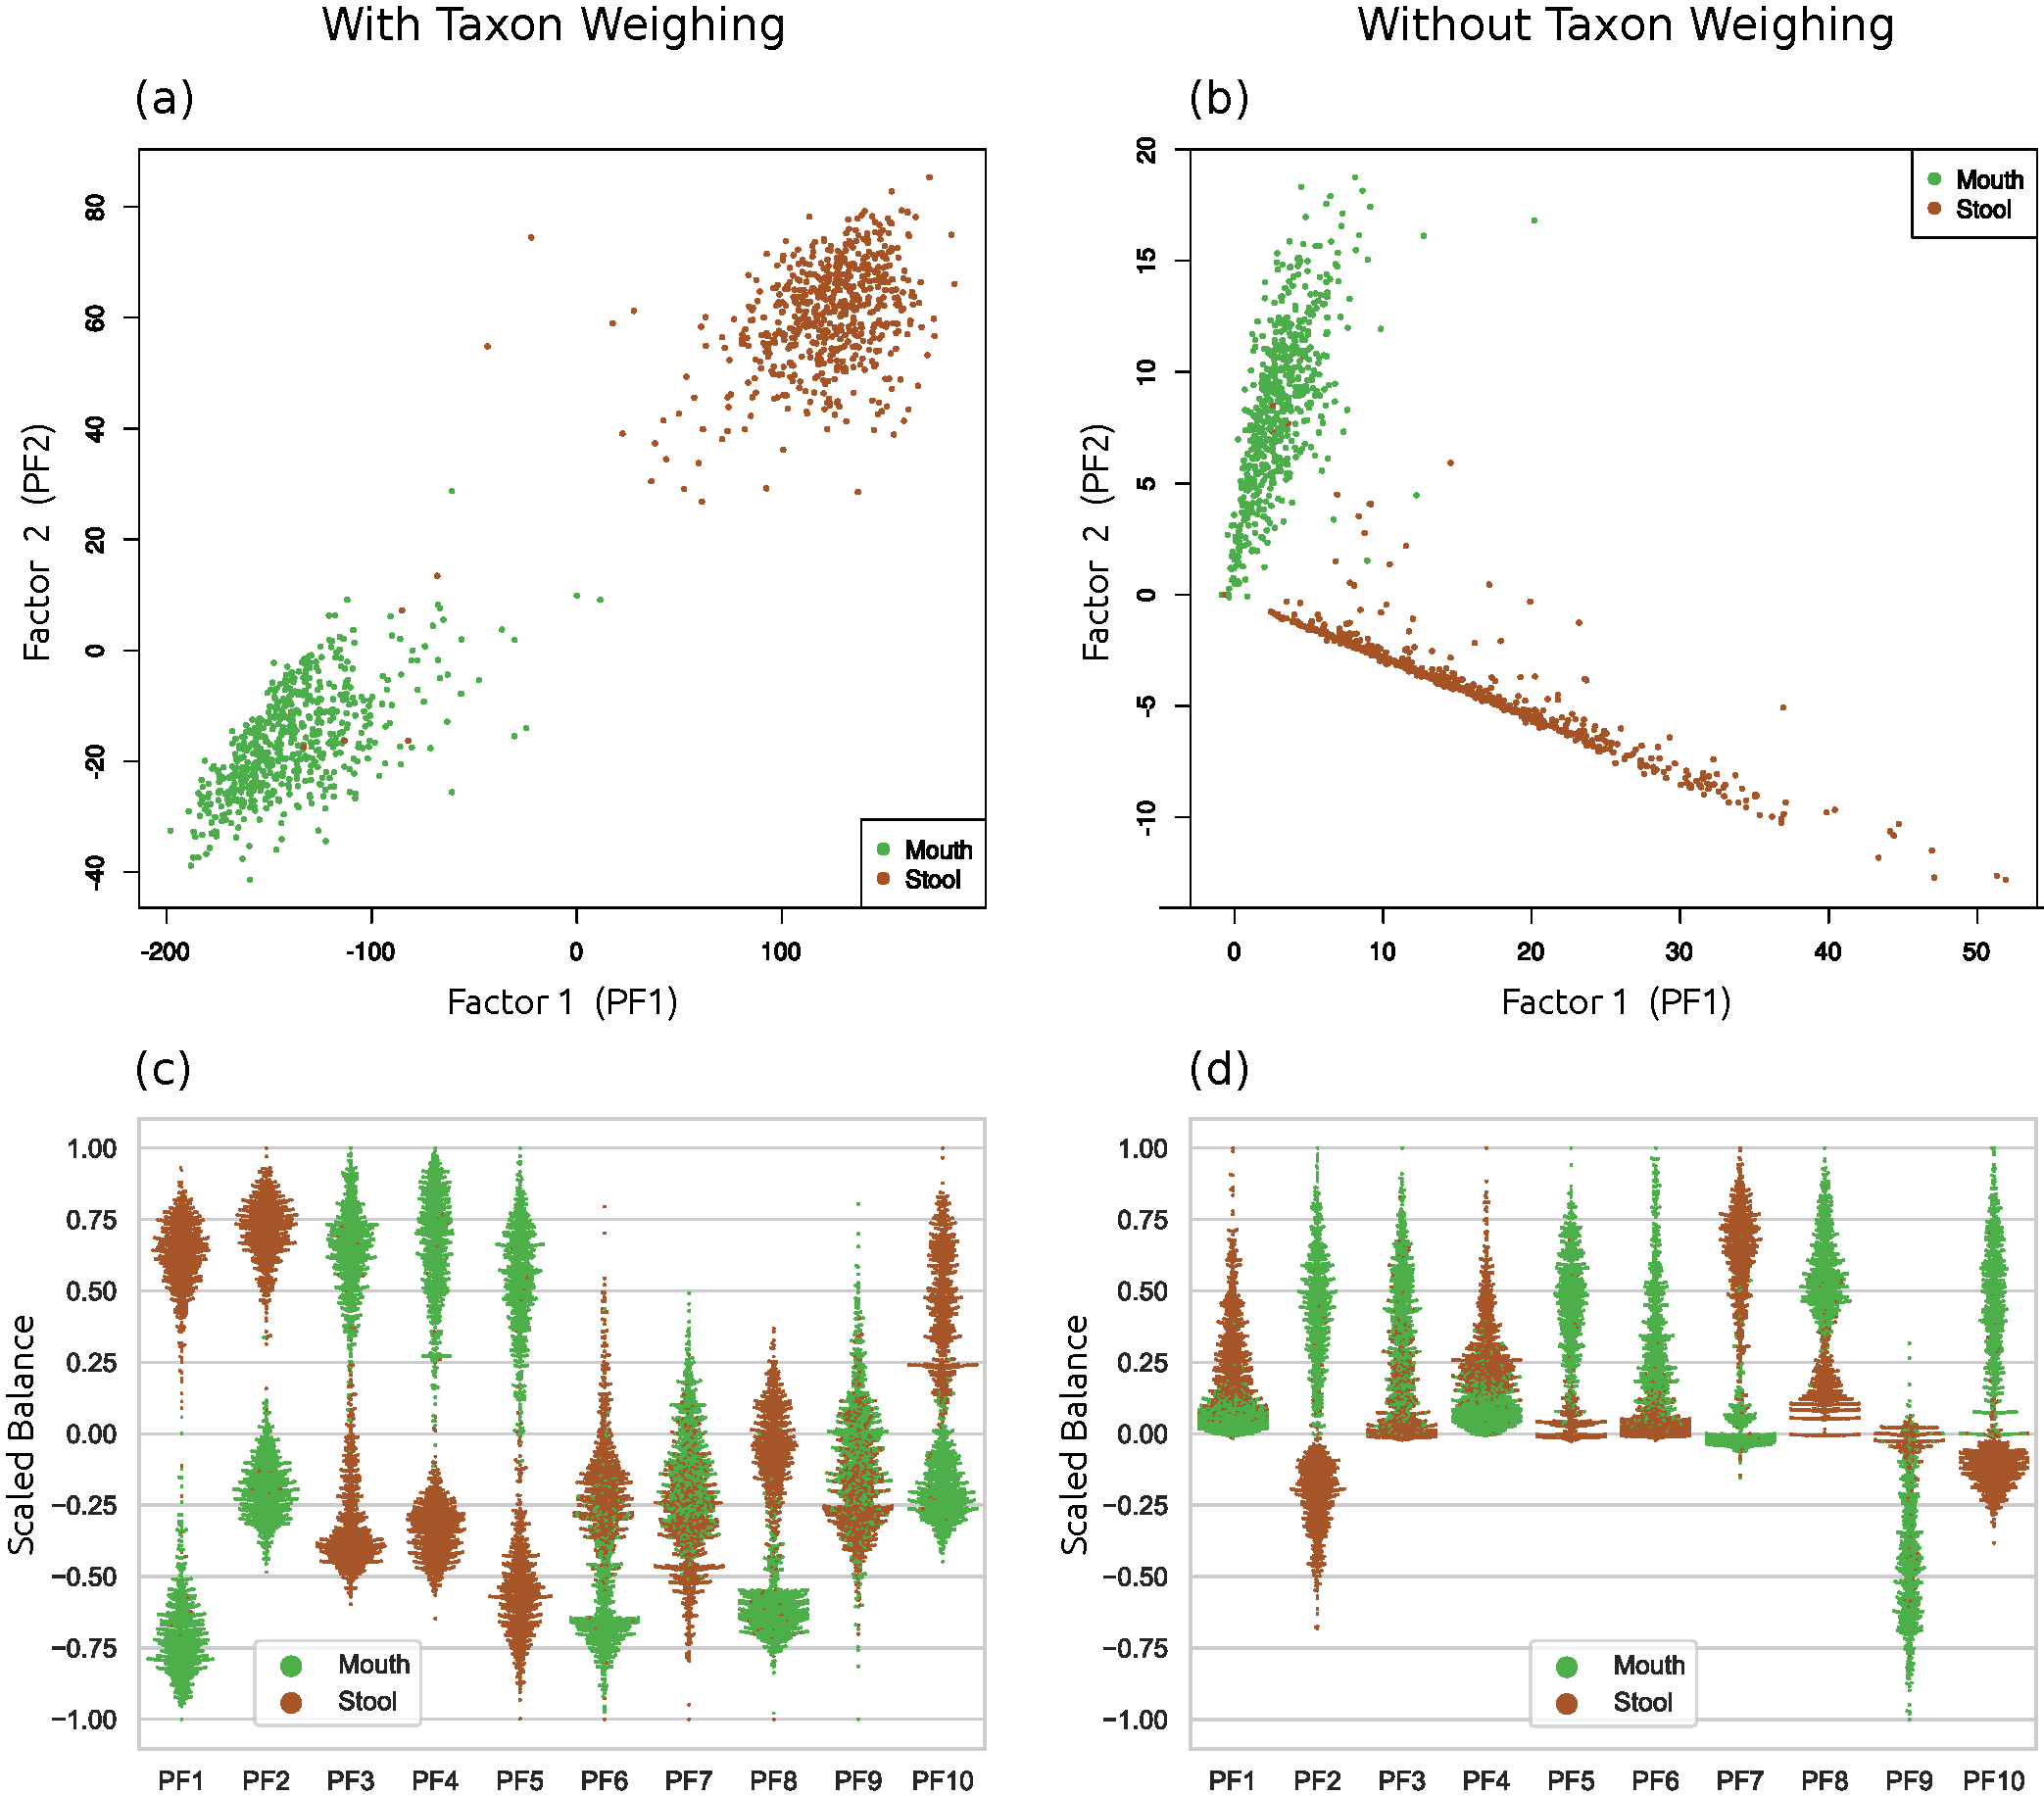
\includegraphics[width=\linewidth]{pdf/hmp_pf_of_600_factor_ordination.pdf}
    \begin{subfigure}{0pt}
        \phantomcaption
        \label{fig:hmp_pf_of_600_factor_ordination:sub:2d_with_taxon_weighting}
    \end{subfigure}
    \begin{subfigure}{0pt}
        \phantomcaption
        \label{fig:hmp_pf_of_600_factor_ordination:sub:2d_without_taxon_weighting}
    \end{subfigure}
    \begin{subfigure}{0pt}
        \phantomcaption
        \label{fig:hmp_pf_of_600_factor_ordination:sub:10d_with_taxon_weighting}
    \end{subfigure}
    \begin{subfigure}{0pt}
        \phantomcaption
        \label{fig:hmp_pf_of_600_factor_ordination:sub:10d_without_taxon_weighting}
    \end{subfigure}
    \caption[Ordination of an oral/fecal subset of the \acs{HMP} dataset]{
        \textbf{Ordination of an oral/fecal subset of the \ac{HMP} dataset.}
        The figure shows the ordination-visualization of factors found by Placement-Factorization
        on our oral/fecal subset of the \ac{HMP} dataset.
        In \subref{fig:hmp_pf_of_600_factor_ordination:sub:2d_with_taxon_weighting}
        and \subref{fig:hmp_pf_of_600_factor_ordination:sub:2d_without_taxon_weighting},
        we show the balances at the winning edges of the first two factors, colorized by the body site of each sample,
        with and without taxon weighting.
        \\
        Moreover, in order to examine how well further factors of later iterations split the data,
        we here employ a visualization of phylofactors, which we call \emph{balance swarm plots},
        by plotting the balances of each factor individually.
        This type of per-factor visualization is similar to, e.\,g., Figure~4 of \cite{Washburne2019}.
        Subfigures \subref{fig:hmp_pf_of_600_factor_ordination:sub:10d_with_taxon_weighting} and
        \subref{fig:hmp_pf_of_600_factor_ordination:sub:10d_without_taxon_weighting} show the first ten factors
        (PF1--PF10), again with and without taxon weighting, respectively.
        These can be understood as multi-dimensional scatter plots, where each dimension is shown separately:
        Each column corresponds to a factor, with the vertical axis being the balances,
        and horizontal space within each column used to spread samples at nearby positions,
        revealing their distribution density.
        That is, the first two columns of
        \subref{fig:hmp_pf_of_600_factor_ordination:sub:10d_with_taxon_weighting} and
        \subref{fig:hmp_pf_of_600_factor_ordination:sub:10d_without_taxon_weighting}
        correspond to the scatter plots of
        \subref{fig:hmp_pf_of_600_factor_ordination:sub:2d_with_taxon_weighting}
        and \subref{fig:hmp_pf_of_600_factor_ordination:sub:2d_without_taxon_weighting}, respectively.
%         the balances were scaled by $ \max(~ |\min|, |\max| ~) $ to bring them into the $[ -1.0, 1.0 ]$ interval,
%         without losing the centering around \num{0}, to for comparability
        The balances were scaled to bring them into the $[ -1.0, 1.0 ]$ interval for better comparability across factors,
        while keeping the centering at \num{0}.
%         Subfigure \subref{fig:hmp_pf_of_600_factor_ordination:sub:10d_with_taxon_weighting}
% %         is identical to \figref{fig:hmp_pf:sub:of_600_swarm} of the main text, and 
%         shows that almost all factors individually suffice to separate the data by body site;
%         in \subref{fig:hmp_pf_of_600_factor_ordination:sub:10d_without_taxon_weighting},
%         the separation is still present, but not as distinguished.
%         \\
%         \todo{See also ref to table listing our and their split taxa}
%         \todo{make it more clear which factor corresponds to which clade}
    }
    \label{fig:hmp_pf_of_600_factor_ordination}
\end{figure}

\figref{fig:hmp_pf_of_600_factor_ordination} indicates that most factors found by our Placement-Factorization
are indeed capable of separating body sites from each other.
In particular, \figref{fig:hmp_pf_of_600_factor_ordination:sub:2d_with_taxon_weighting}
exhibits a clear separation of the two body sites, similar to Figure~S3 of \citeay{Washburne2017a}.
Furthermore, \figref{fig:hmp_pf_of_600_factor_ordination:sub:10d_with_taxon_weighting}
shows that almost all factors individually suffice to separate the data by body site:
eight out of the first ten factors found by Placement-Factorization \emph{with} taxon weighting
clearly separate the oral from the fecal samples.
The remaining two factors (PF7 and PF9) separate most of the samples,
but also have an interval of balances that contains samples from both body sites.
Placement-Factorization \emph{without} taxon weighting also separates samples based on their body site,
as shown in \figref{fig:hmp_pf_of_600_factor_ordination:sub:10d_without_taxon_weighting},
but with a less clear distinction.
This is also obvious from the ordination scatter plots
shown in \figref{fig:hmp_pf_of_600_factor_ordination:sub:2d_without_taxon_weighting}.

% in \figref{fig:hmp_pf_of_600_factor_ordination:sub:10d_without_taxon_weighting},
% the separation is still present, but not as distinguished.

% \begin{figure}[hbtp!]
%     \centering
% %      \includegraphics[width=\linewidth]{pdf/hmp_pf.pdf}
%     \begin{subfigure}{0pt}
%         \phantomcaption
%         \label{fig:hmp_pf:sub:of_600_swarm}
%     \end{subfigure}
%     \begin{subfigure}{0pt}
%         \phantomcaption
%         \label{fig:hmp_pf:sub:all_violin}
%     \end{subfigure}
%     \caption[Ordination of Placement-Factorization of the \acs{HMP} dataset]{
%         \textbf{Ordination of Placement-Factorization of the \ac{HMP} dataset.}
%         In this visualization of phylogenetic factors,
%         we show the balances of the winning edge at different factors for all samples.
%         \\
%         Subfigure \subref{fig:hmp_pf:sub:of_600_swarm} shows the first \num{10} factors
%         found by Placement-Factorization with taxon weighting on the oral/fecal subset of the \ac{HMP} dataset.
%         We call this a \emph{balance swarm plot}.
%         It can be understood as multi-dimensional scatter plot, where each dimension is shown separately:
%         Each column corresponds to a factor (PF1--PF10), with the vertical axis being the balances,
%         and horizontal space within each column used to spread samples at nearby positions,
%         revealing their distribution density.
%         The balances were scaled to the $[-1.0, 1.0]$ interval for better comparability across factors,
%         while keeping the centering at \num{0}.
%         \\
%         Subfigure \subref{fig:hmp_pf:sub:all_violin} shows the first factor of Placement-Factorization with taxon weighting
%         on the full \ac{HMP} dataset.
%         The violin plots in \subref{fig:hmp_pf:sub:all_violin} extend on the idea of balance swarm plots
%         by separating different groups of samples, based on their body site.
%         This allows to clearly see the distribution of balances at the factor for all groups of samples.
%         \\
%         The exhaustive versions of these plots, with and without taxon weighting, and for more factors,
%         are shown in the context of the typical two- and three-dimensional scatter plots in
%         \figref{fig:hmp_pf_of_600_factor_ordination}, \figref{fig:hmp_pf_all_ordination}, and
%         \figref{fig:hmp_pf_all_violins}.
%         See there for more details.
%     }
%     \label{fig:hmp_pf}
% \end{figure}

% ----------------------------------------------------------------------------------------------------------------------
%     HMP Dataset
% ----------------------------------------------------------------------------------------------------------------------

\subsection{Full HMP dataset}
\label{ch:Factorization:sec:Evaluation:sub:FullHMPDataset}

% ------------------------------------------------
%     Full Dataset
% ------------------------------------------------

% \paragraph{Full Dataset}
% \label{sec:Factorization:sub:Evaluation:sub:FullHMPDataset:par:FullDataset}

% We moreover used the full \ac{HMP} dataset to conduct some in-depth analyses of our adaptation,
% and to showcase some novel types of visualizations.

Finally, we conducted Placement-Factorization on the whole \ac{HMP} dataset with all \num{9192} samples,
instead of just the oral/fecal subset,
in order to evaluate how the method performs on large datasets with more than two categories (body sites) to distinguish.
See \tabref{tab:hmp_data_overview} for an overview of the samples, as well as a list of the eight body site labels
that we used for classifying the samples.
We here do not discuss the taxa that were split by each factor,
as such an in-depth biological discussion is beyond the scope of this work.
Instead, we evaluate how well different body sites were separated by the factors.
To this end, we show ordination plots of the first two and three factors in \figref{fig:hmp_pf_all_ordination}.

\begin{figure}[!htbp]
    \centering
     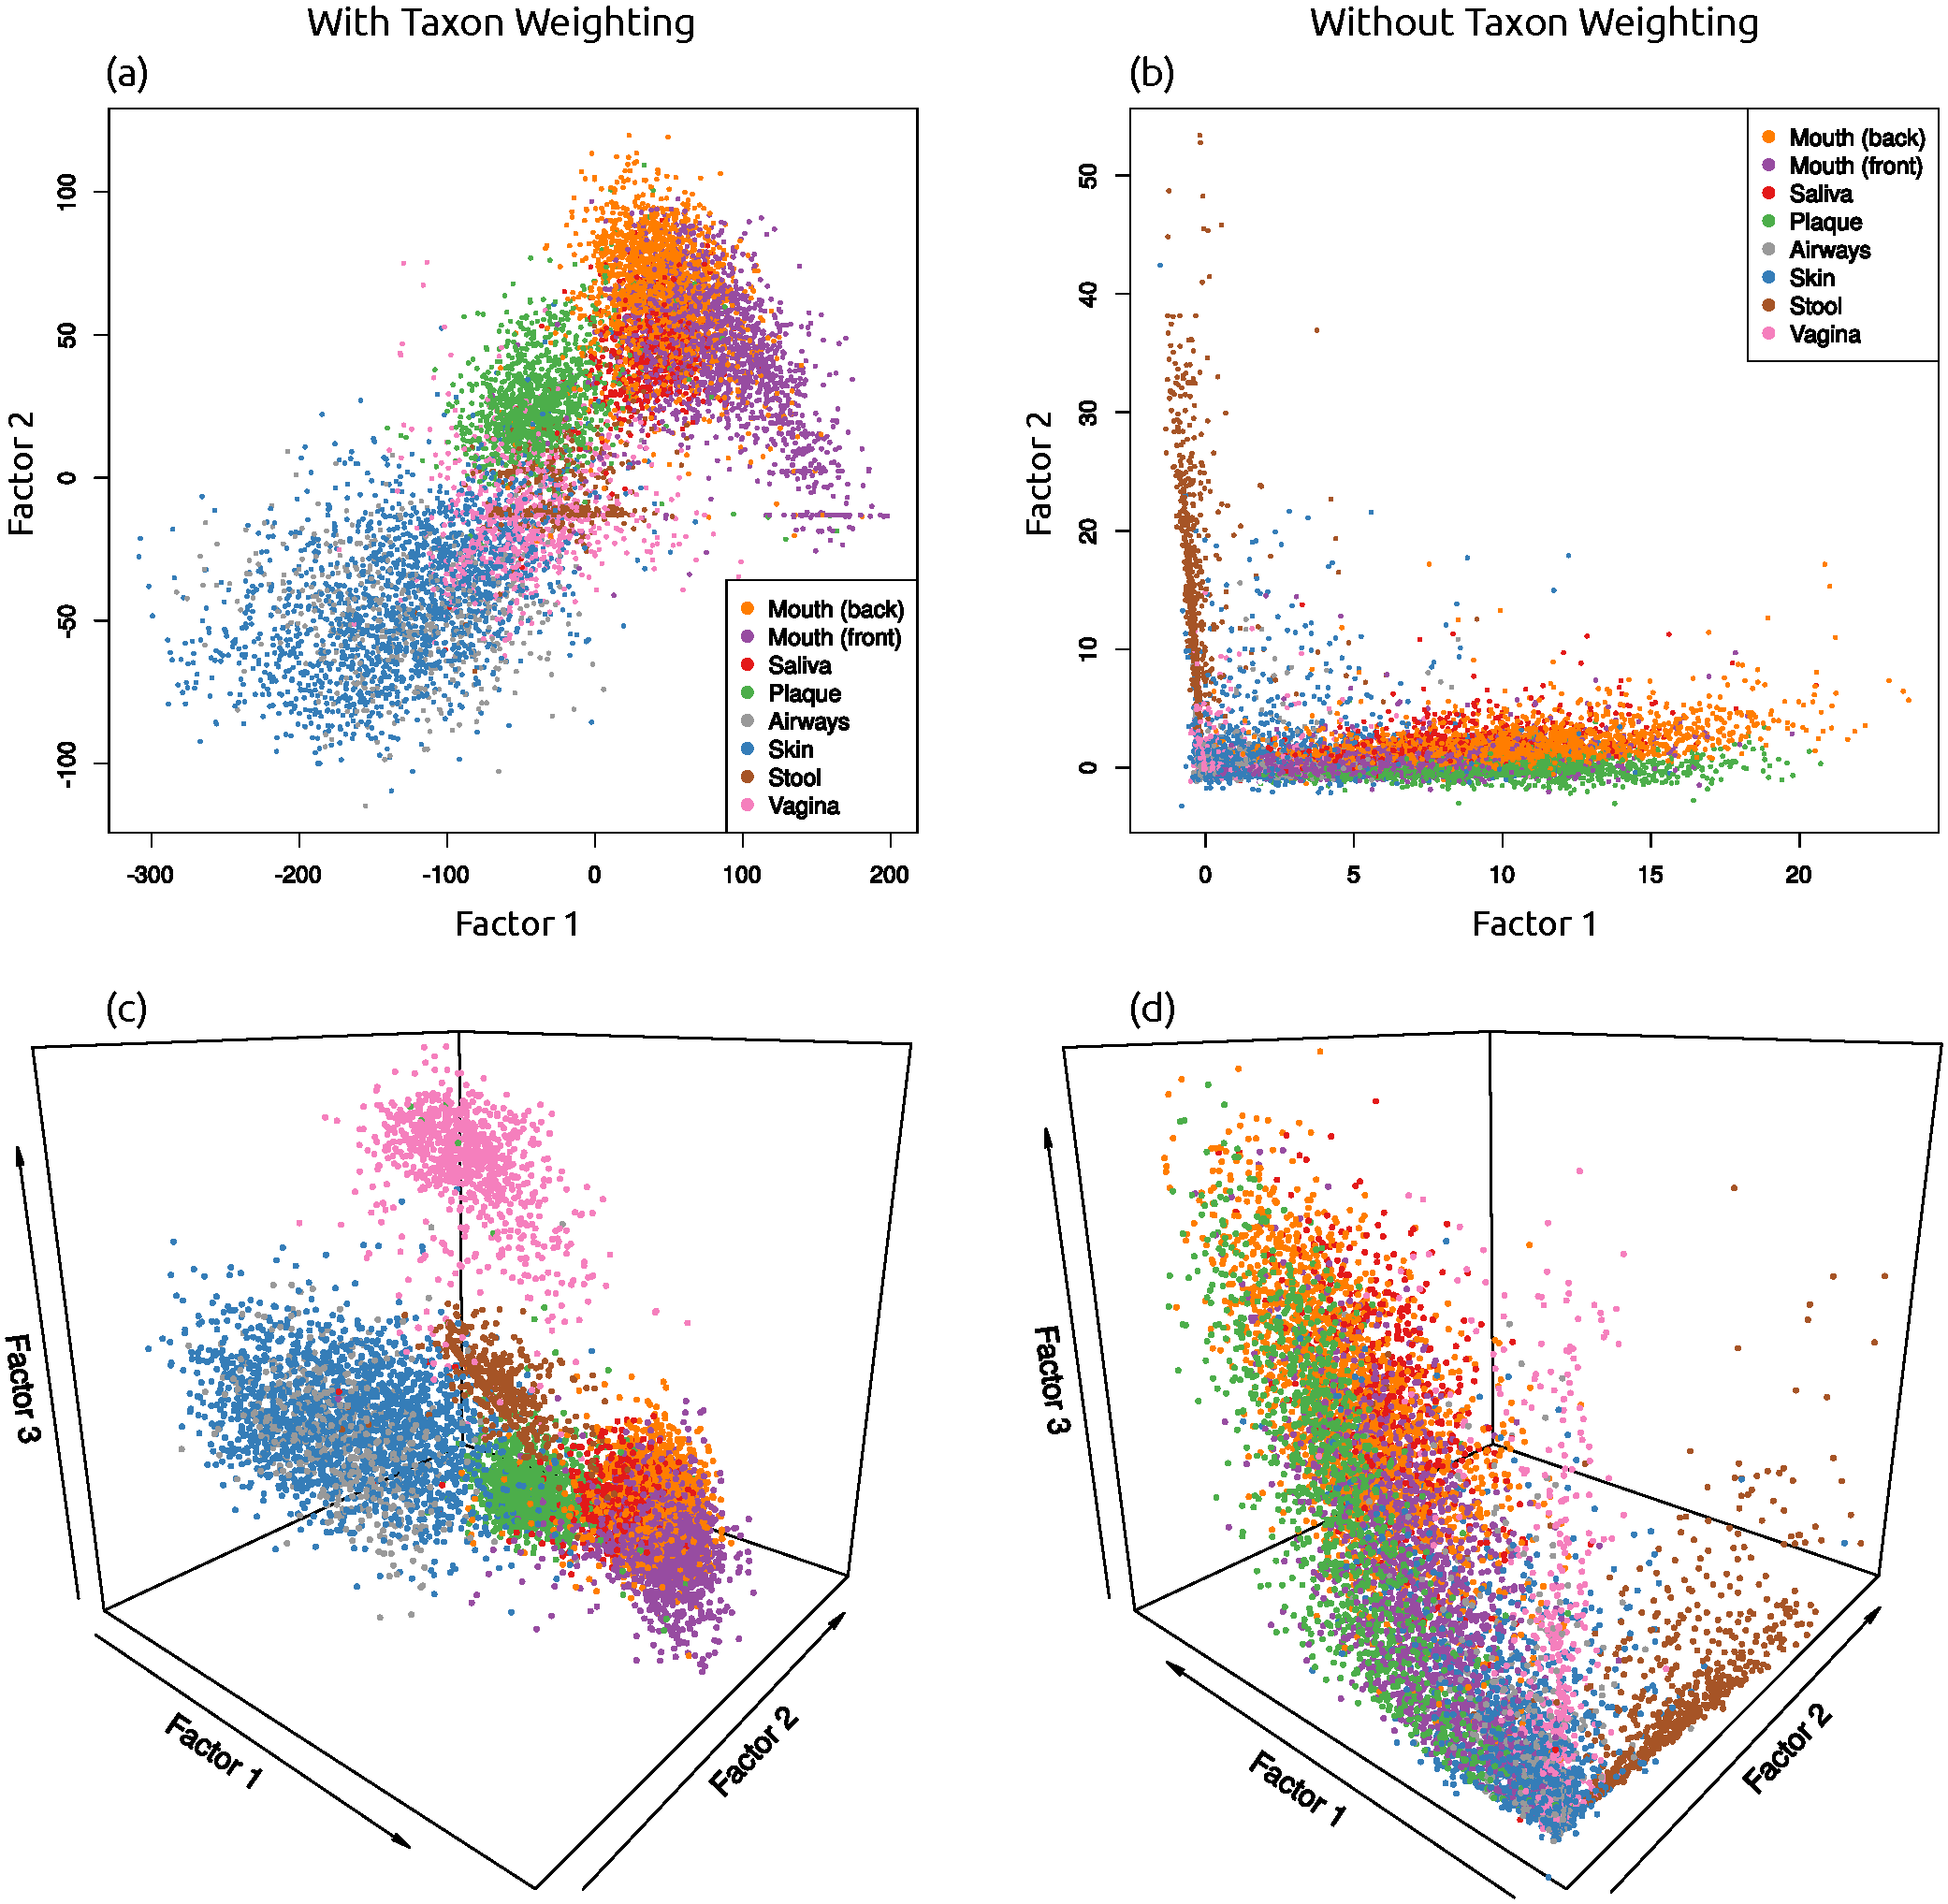
\includegraphics[width=\linewidth]{pdf/hmp_pf_all_ordination.pdf}
    \begin{subfigure}{0pt}
        \phantomcaption
        \label{fig:hmp_pf_all_ordination:sub:2d_with_taxon_weighting}
    \end{subfigure}
    \begin{subfigure}{0pt}
        \phantomcaption
        \label{fig:hmp_pf_all_ordination:sub:2d_without_taxon_weighting}
    \end{subfigure}
    \begin{subfigure}{0pt}
        \phantomcaption
        \label{fig:hmp_pf_all_ordination:sub:3d_with_taxon_weighting}
    \end{subfigure}
    \begin{subfigure}{0pt}
        \phantomcaption
        \label{fig:hmp_pf_all_ordination:sub:3d_without_taxon_weighting}
    \end{subfigure}
    \caption[Ordination of Placement-Factorization of the full \acs{HMP} dataset]{
        \textbf{Ordination of Placement-Factorization of the full \ac{HMP} dataset.}
%         In \figref{fig:hmp_pf_of_600_factor_ordination},
%         we use an oral/fecal subset of the \ac{HMP} dataset \cite{Huttenhower2012,Methe2012}
%         to compare Placement-Factorization to a case study of the original Phylofactorization.
%         Here, we instead used the whole \ac{HMP} dataset,
        Here, we use the whole \ac{HMP} dataset,
        labeled by \num{8} body site regions as listed in \tabref{tab:hmp_data_overview},
        to asses how well Placement-Factorization with a \ac{GLM} objective function
        can separate samples based on their body site label.
%         Labels are encoded as factor levels, creating dummy variables, using GLM.
        The figure again shows the balances of the winning edges of the first two and three factors, respectively,
        with and without taxon weighting.
    }
    \label{fig:hmp_pf_all_ordination}
\end{figure}

These plots already reveal that Placement-Factorization indeed separates samples from each other based on their body site.
However, given the eight body site labels that we used, these plots are overloaded and hard to read.
Hence, we extended on the idea of balance swarm plots (as introduced above for the oral/fecal subset)
by separating them into individual plots per factor,
each showing the balance distribution of groups of samples based on their respective body site.
This allows to clearly see the distribution of balances at the factor for all groups of samples.
An example for the first four factors is shown in \figref{fig:hmp_pf_all_violins}.

\begin{figure}[!htpb]
    \centering
     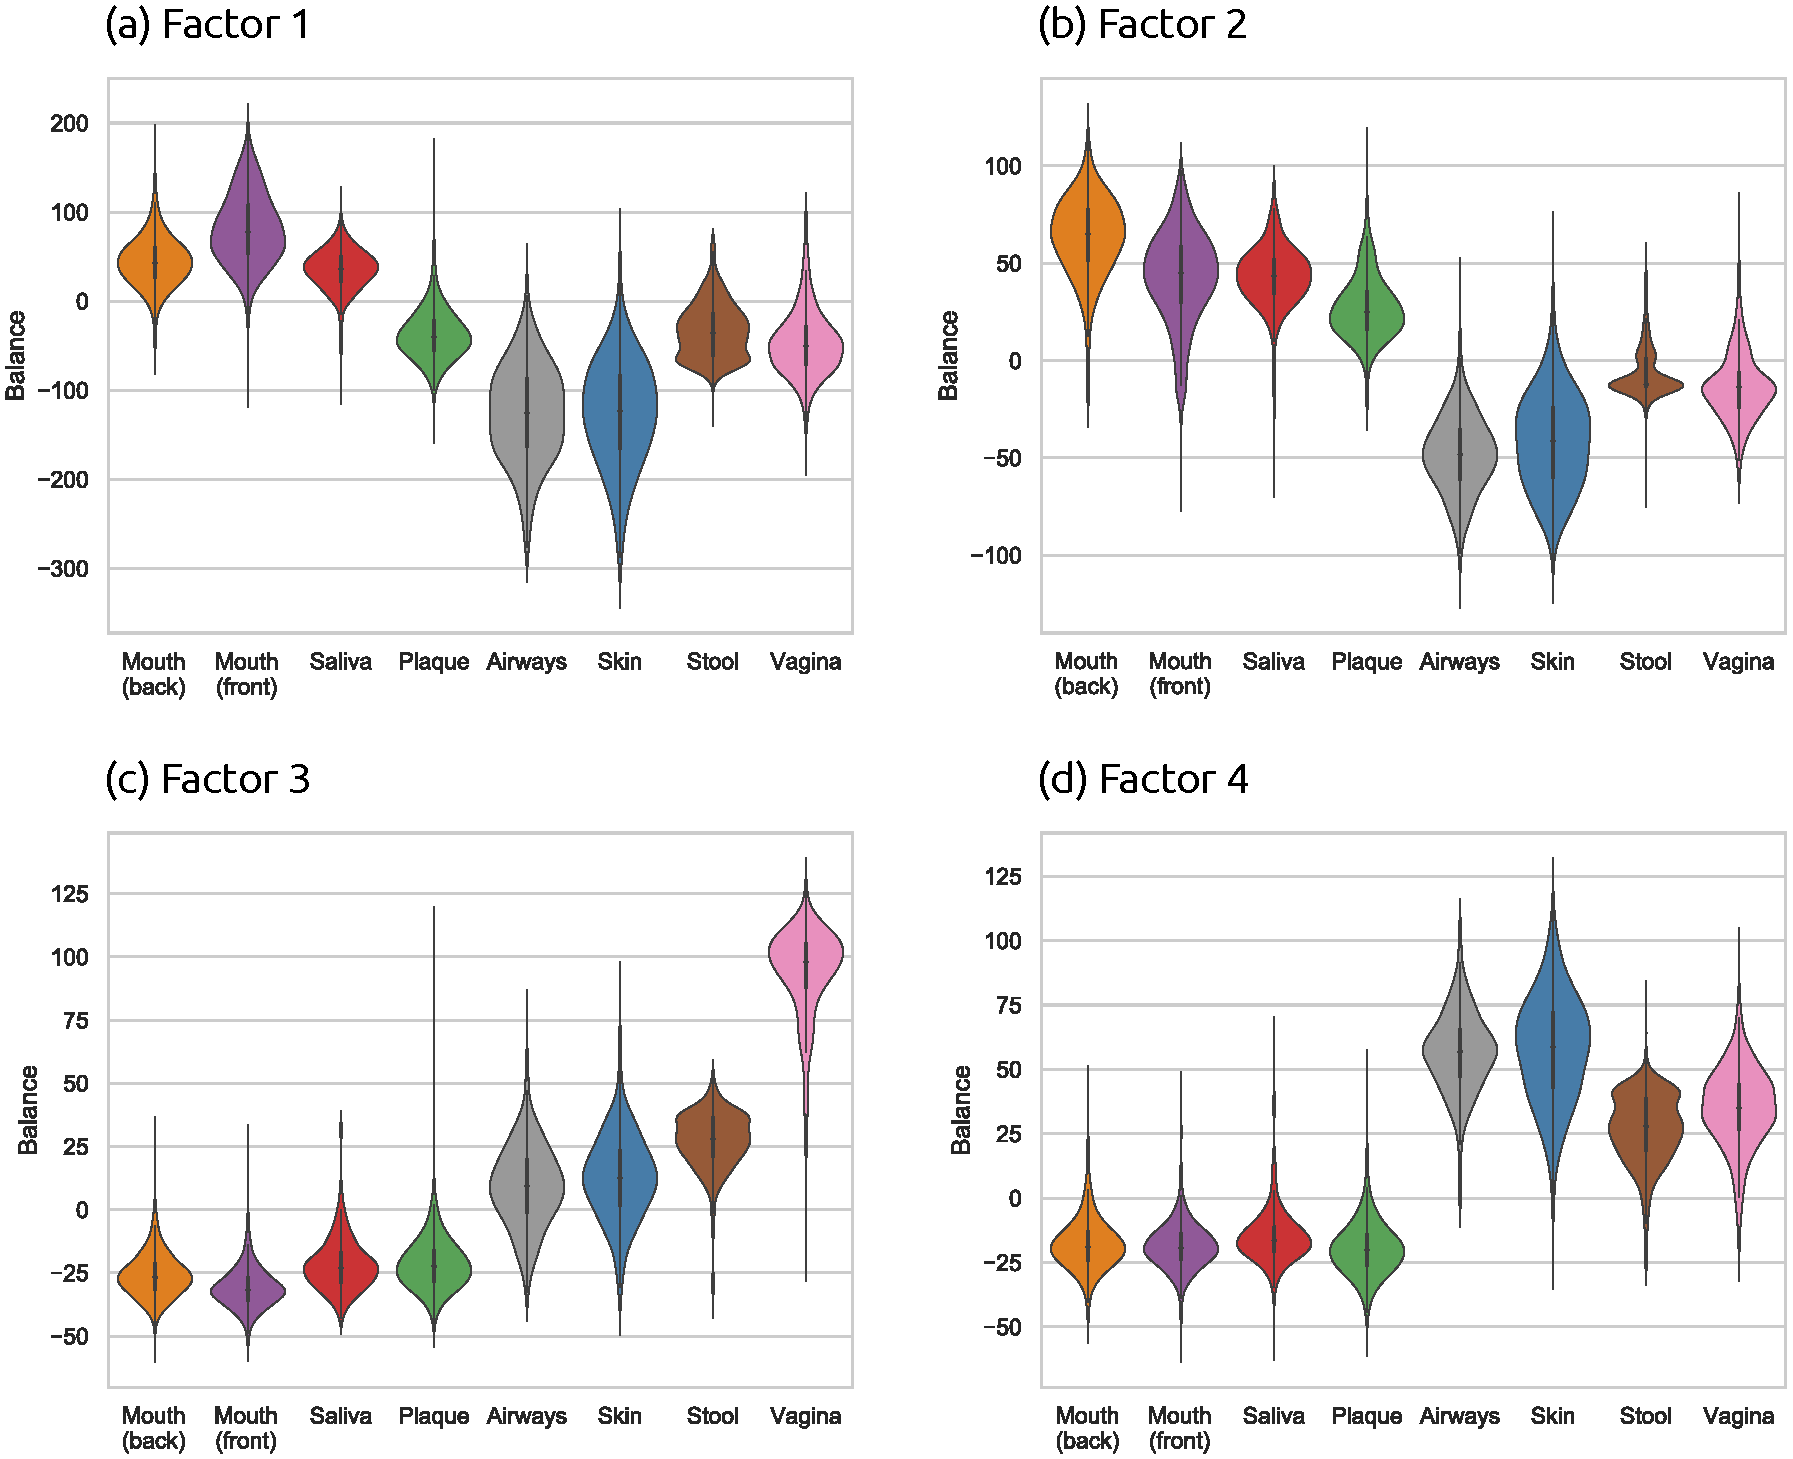
\includegraphics[width=\linewidth]{pdf/hmp_pf_all_violins.pdf}
    \begin{subfigure}{0pt}
        \phantomcaption
        \label{fig:hmp_pf_all_violins:sub:factor_1}
    \end{subfigure}
    \begin{subfigure}{0pt}
        \phantomcaption
        \label{fig:hmp_pf_all_violins:sub:factor_2}
    \end{subfigure}
    \begin{subfigure}{0pt}
        \phantomcaption
        \label{fig:hmp_pf_all_violins:sub:factor_3}
    \end{subfigure}
    \begin{subfigure}{0pt}
        \phantomcaption
        \label{fig:hmp_pf_all_violins:sub:factor_4}
    \end{subfigure}
    \caption[Ordination of the first four factors of the \acs{HMP} dataset]{
        \textbf{Ordination of the first four factors of the \ac{HMP} dataset.}
        The balance swarm plots as shown in
        \figref{fig:hmp_pf_of_600_factor_ordination:sub:10d_with_taxon_weighting} and
        \figref{fig:hmp_pf_of_600_factor_ordination:sub:10d_without_taxon_weighting}
        allow for a more detailed understanding of how each factor separates the samples.
        They can be colored by either continuous meta-data variables, similar to Figure~5(a) of \citeay{Washburne2017a},
        or a categorical variable with a limited number of categories, as shown in \figref{fig:hmp_pf_of_600_factor_ordination}.
        However, for the eight body regions that we use for the \ac{HMP} data,
        this type of visualization becomes hard to inspect visually.
        Hence, we here extend on the idea of balance swarm plots,
        and show the distribution of balances for each factor and for each body sites separately.
        \\
        The data shown here is the result of Placement-Factorization with taxon weighting on the full \ac{HMP} dataset.
        Each subfigure here shows the balances of the winning edge of a factor,
        grouped by the categorical meta-data variable body site.
        That is, the subfigures correspond to the scatter plots of the first two and three factors
        shown in \figref{fig:hmp_pf_all_ordination}.
        In other words, each subfigure here represents a disentangled column of a balance swarm plot,
%         e.\,g., \figref{fig:hmp_pf_of_600_factor_ordination:sub:10d_with_taxon_weighting},
%         with eight instead of just two body sites,
        where each body site is displayed separately by its own violin. %in order to better distinguish between them.
%         Subfigure \subref{fig:hmp_pf_all_violins:sub:factor_1} is identical to \figref{fig:hmp_pf:sub:all_violin}
%         of the main text, and included here for comparability.
    }
    \label{fig:hmp_pf_all_violins}
\end{figure}

The visualizations shown in \figref{fig:hmp_pf_all_ordination} and \figref{fig:hmp_pf_all_violins}
indicate that Placement-Factorization separates samples mainly based on the distinction oral vs.~remaining body sites,
with a further separation of plaque samples in the oral region.
This can, for example, be seen in \figref{fig:hmp_pf_all_violins:sub:factor_1},
where the first three groups ``Mouth (back)'', ``Mouth (front)'', and ``Saliva'' exhibit balances above \num{0},
while all other groups have balances below \num{0}.
Further factors then separate vaginal samples and skin and airways samples from the rest of the samples,
as shown in \figref{fig:hmp_pf_all_violins:sub:factor_2}--\subref{fig:hmp_pf_all_violins:sub:factor_4}.

As shown in \figref{fig:pf_bv_place_ilr_ordination} and \figref{fig:hmp_pf_of_600_factor_ordination} before,
the plots \emph{with} taxon weighting form ``clouds'',
whereas the plots \emph{without} taxon weighting form an ``L''-shape.
In all cases, a separation of the oral samples from the other regions is clearly visible.
Noticeably, in \figref{fig:hmp_pf_all_ordination:sub:2d_with_taxon_weighting},
a part of the stool and mouth samples form a horizontal line,
which indicates that the second factor does not distinguish between samples from those regions.
It is striking that the samples from the vaginal region in
\figref{fig:hmp_pf_all_ordination:sub:2d_with_taxon_weighting} and
\subref{fig:hmp_pf_all_ordination:sub:3d_with_taxon_weighting} are not separated from the other samples
until the third factor, which is visible as a pink cloud above the rest of the samples
in \figref{fig:hmp_pf_all_ordination:sub:3d_with_taxon_weighting}.
This again serves as a caveat that one needs to consider enough factors
in order to get a complete understanding of the results.

This can be seen in more detail in \figref{fig:hmp_pf_all_violins}.
In all subfigures, the oral regions are separated from the other regions:
For example, in \figref{fig:hmp_pf_all_violins:sub:factor_1},
mouth and saliva samples exhibit balances above \num{0}, in contrast to all other samples.
In \figref{fig:hmp_pf_all_violins:sub:factor_2}--\subref{fig:hmp_pf_all_violins:sub:factor_4},
the plaque samples join the other oral samples in terms of their balance values.
In \figref{fig:hmp_pf_all_violins:sub:factor_2}, the stool samples have a distinct bulge near \num{0},
which corresponds to the horizontal line (factor 2)
in \figref{fig:hmp_pf_all_ordination:sub:2d_with_taxon_weighting}.
Furthermore, the third factor in \figref{fig:hmp_pf_all_violins:sub:factor_3}
again clearly separates the vaginal samples from the rest,
corresponding to the pink cloud in \figref{fig:hmp_pf_all_ordination:sub:3d_with_taxon_weighting}.

Overall, Placement-Factorization can distinguish the \ac{HMP} samples by body site,
at least to the extent that can expected from abundance differences in the samples.
For example, it would be unrealistic to expect the algorithm to perfectly separate samples
from the back and front of the mouth from each other,
as their microbial compositions are expected to be highly similar.

% ----------------------------------------------------------------------------------------------------------------------
%     Performance
% ----------------------------------------------------------------------------------------------------------------------

\subsection{Performance}
\label{ch:Factorization:sec:Evaluation:sub:Performance}

The run time of Placement-Factorization depends on
(a) the number of input samples, (b) the number of branches of the reference tree, and (c) the number of iterations to run.
As the computations are conducted on the mass matrix instead of single placements,
the performance and memory requirements of Placement-Factorization are independent
from the total number of sequences/placements in the dataset.
% these however do influence the initial reading of the input files.
In each iteration, and for each edge of the tree (except the ones that won previous factors),
the balances of all samples are computed, and the objective function is evaluated.
In case of using a \ac{GLM} to express the relationship of balances with meta-data,
this involves fitting a model across all samples.
In our implementation, all these computations are parallelized.

Our relatively small \ac{BV} test dataset ran on a standard laptop with \num{4} cores,
taking \SI{30}{\second} per iteration.
The full \ac{HMP} dataset with \num{9 192} samples and our reference tree with \num{3 825} branches
required \SI{13.0}{\giga\byte} of memory in our non-optimized prototype implementation,
as took less than \SI{90}{\second} per iteration using \num{20} cores.
Also, note that each iteration splits away a clade of the tree;
later iterations thus become faster,
as the sizes of the subtrees within which the balances need to be computed get smaller each time.
% as the splitting of the tree into subtrees reduces the number of edges
% that need to be taken into account in each balance computation.
Hence, we conclude that Placement-Factorization is well suited even for very large datasets.

% ######################################################################################################################
%         Summary and Outlook
% ######################################################################################################################

\section{Summary and Outlook}
\label{ch:Factorization:sec:SummaryOutlook}

In this chapter, we presented an adaption of Phylofactorization \cite{Washburne2017a,Washburne2019}
to phylogenetic placement data, which we call \emph{Placement-Factorization}.
Placement-Factorization identifies branches of the reference tree, called \emph{phylogenetic factors},
that exhibit a relationship with environmental meta-data features, that is,
branches along which putative functional traits might have arisen in conjunction with changes in environmental variables.
This factorization of the tree can be used as an ordination tool to visualize
how samples are separated by changes along the factors,
and as a dimensionality-reduction tool \cite{Washburne2017a}.
It thus complements Edge Correlation (see \secref{ch:Visualization:sec:Methods:sub:EdgeCorrelation}), %that identifies branches
% that drive patterns and relationships between samples and their environmental meta-data variables,
but further allows to identify nested dependencies within sub-clades of the reference tree.

% We showed that our adaption yields results that are consistent with previous methods and findings.
% summarize bv results
% In conclusion, Placement-Factorization yields factors of the oral/fecal data
% that are mostly consistent with the findings of Phylofactorization \cite{Washburne2017a},
% and is also able to reasonably separate the samples of larger datasets with several categorical labels.

We contributed novel ideas to Phylofactorization by
(a) adapting the concept to phylogenetic placement,
which can be thought of as placing abundances along branches of the tree instead of just at its tips;
and (b) suggesting a novel visualization for the objective function value at each edge of the reference tree,
which helps in the interpretation of the factors being split in each iteration.
Furthermore, we explored several advantages of using a fixed reference tree instead of a tree inferred from OTUs
in \secref{sec:Factorization:sub:Methods:sub:MethodComparison}.
We leave the adaptation of some of the original concepts of Phylofactorization to phylogenetic placements
as future work, such as binned phylogenetic units (BPUs), stopping criteria for the iterations,
as well as further experimentation with different objective functions and aggregation and contrast functions
\cite{Washburne2017a,Washburne2018}.
Based on our findings and experiments,
we conjecture that these concepts should be readily applicable to our Placement-Factorization.

In contrast to the original Phylofactorization \cite{Washburne2017a}, our implementation also supports
the taxon weigting scheme used in the balances compuation, as explained in \secref{ch:Balances:sec:Methods:sub:EdgeWeights}.
We find that Placement-Factorization \emph{without} taxon weighting
behaves similar to the original Phylofactorization (which also does not employ a taxon weighting scheme),
while Placement-Factorization \emph{with} taxon weighting
yields results that are more in line with our previous results based on edge imbalances
(\secref{ch:Foundations:sec:PhylogeneticPlacement:sub:PlacementProcessing:par:EdgeImbalances}).
The latter is likely because taxon weighting has a similar effect of reducing the influence of low mass branches
(low abundance taxa) as the summation-based aggregation step of imbalances.

As discussed in \secref{ch:Factorization:sec:Evaluation},
we found that both, the original Phylofactorization, as well as our Placement-Factorization,
can split clades that are larger than one would expect from other types of analyses of the data.
Considering the distribution of objective function values, as for instance shown in \figref{fig:pf_bv_place_tw_ovs},
it is likely that such large clades are the result of random variability
along a path of branches that are equally relevant for the factor.
Further research is needed to confirm this.

These findings suggest that it might be beneficial to introduce a significance value for each factor,
which assesses how relevant the particular winning edge is
compared to other edges that yielded a high objective value in an iteration.
This idea is intrinsically connected (pers.~comm.~with A.~Washburne on 2019-03-01)
to the stopping function of the original Phylofactorization \cite{Washburne2017a},
which uses a Kolmogorov-Smirnov (KS) test \cite{Massey1951}
% of the distribution of P-values from analyses of variance of the regressions on candidate ILR coordinates.
to conservatively estimate when a sufficient number of factors have been identified.
Another strongly connected idea is that of confidence regions of the phylogeny,
defined by regions of the tree in which the ``true'' winning edge falls with a certain confidence \cite{Washburne2019}.
Such a significance value for the winning edge might also enable a form of \emph{soft} factorization,
that does not greedily pick one winning edge per iteration.

Furthermore, the paths of high objective values as for example seen in \figref{fig:pf_bv_place_tw_ovs} indicate
that there is a gradient of the objective function along the edges of the tree.
This could be exploited in a gradient-ascending graph-walking algorithm to identify the phylogenetic factors
of extremely large datasets without having to exhaustively evaluate the objective function at every edge
(pers.~comm.~with A.~Washburne on 2019-03-01).
For example, one could start at one or more random edges on the tree,
and ascend along the edges in the direction of the gradient until a local maximum of the objective function is found.

Phylofactorization is a very recent method whose full potential has just begun being explored \cite{Washburne2019}.
% We here introduced our adaptation and described several ideas for future research,
Given the ideas for future research that we outlined here,
we hence conclude that more work is needed in order to fully reach that potential.

% novel idea:
%
% use parts of the tree that are split by a factor as separate subtrees that can be subjected to visualizations such as edge correlation
% in order to find subtree correlation etc.


% Furthermore, the balance swarm and violin plots as e.\,g. shown in \figref{fig:hmp_pf}
% and (c) suggesting the swarm and violin plots as a more elaborate and multi-dimensional way of visualizing
% the effect of balances at each factor on the separation of samples by their meta-data variables.

% this might be because imbalances are implicitly more robust to the influence of low abundant tax:
% arithmetic mean is more sensitive to large values, which is what we want here,
% while geom mean ...
% https://medium.com/@JLMC/understanding-three-simple-statistics-for-data-visualizations-2619dbb3677a
% ar mean is well suited for additive data, which we have if we look at masses per branch.
% more sensitive to large values, which is what we want.
% https://towardsdatascience.com/on-average-youre-using-the-wrong-average-geometric-harmonic-means-in-data-analysis-2a703e21ea0
% see also \figref{fig:bv_place_edge_balances_correlation:sub:without_taxon_weighting},
% where balances without taxon weighting clearly are too sensitive for the low abundance clades!
% and see what we discussed above about taxon splitting

% corr can only show first component, cf bv figure xy.
% phylofactor can also reveal corr/dependencies on deeper levels/different components/factors.
% ov figure: only magnitue. if we consider the glm fit as a correlation, we do not seenot direction of the correlation here...
% OV tends to decrease with every iteration (no much more can be explained). note this, and add the column to the table maybe.
% see BV phylo facotr.log file for OVs that behave like this
% variance - PhyCA: see biorxiv preprint ll 450!
